\documentclass[aspectratio=169]{beamer}
% Theme Setup (Clean and Professional)
\usetheme{Madrid}
\usecolortheme{beaver}

% Preamble Configuration
\usepackage[T1]{fontenc}
\usepackage{lmodern}
\usepackage{amsmath, amssymb}
\usepackage{listings}
\usepackage{graphicx}
\usepackage{booktabs}
\usepackage{xcolor}
\usepackage{multirow}
\usepackage{comment}
\usepackage{tikz}
\usetikzlibrary{shapes, shapes.geometric, arrows, positioning, arrows.meta, patterns}
\usepackage{pgfplots}
\pgfplotsset{compat=1.18}

% Unified TikZ Styles
\tikzset{
  feasible area/.style={fill=blue!12, opacity=0.75},
  fixed cost area/.style={fill=red!10, opacity=0.7},
  constraint line/.style={thick, blue!70!black},
  objective line/.style={dashed, orange!85!black, very thick},
  integer point/.style={mark=*, only marks, mark options={fill=red!70!black, scale=0.85}},
  lp optimal/.style={fill=green!60!black, diamond, inner sep=2.2pt},
  ilp optimal/.style={fill=red!70!black, star, star points=5, inner sep=2.2pt},
  milp optimal/.style={fill=red!70!black, star, star points=5, inner sep=2.5pt},
  fixed cost point/.style={fill=black, circle, inner sep=1.8pt},
  bnb node/.style={rectangle, rounded corners=3pt, draw=black!70, thick, align=left, inner sep=4pt, font=\scriptsize, fill=white},
  bnb edge/.style={-Stealth, thick, draw=black!75},
  bnb yes/.style={draw=green!60!black, very thick},
  bnb no/.style={draw=red!70!black, dashed, very thick},
}

% Clean Python Listing Style for PuLP 4.0
\lstset{
  language=Python,
  basicstyle=\fontsize{6pt}{7.2pt}\selectfont\ttfamily,
  keywordstyle=\color{blue!75!black}\bfseries,
  stringstyle=\color{red!70!black},
  commentstyle=\color{green!50!black}\itshape,
  backgroundcolor=\color{gray!6},
  frame=single,
  rulecolor=\color{gray!35},
  showstringspaces=false,
  columns=fullflexible,
  keepspaces=true,
  breaklines=true,
  aboveskip=2pt,
  belowskip=2pt
}

% Custom Block Style for Constraints
\newenvironment{constraintblock}[1]{
    \begin{block}{Constraint Rule: #1}
    \vspace{-0.3em}
}{
    \end{block}
}

\title{Introduction to Integer Linear Programming}
\subtitle{BUS 104: Decision Analysis and Management Science}
\author{Danko Turcic}
\titlegraphic{\includegraphics[width=5cm]{UCR-Logo.jpg}}

\begin{document}

% Title Frame
\begin{frame}[noframenumbering,plain]
  \maketitle
\end{frame}

% ----------------------------------------------------------------------
% SLIDE 2: Agenda - ILPs Introduced in Class
% ----------------------------------------------------------------------
\begin{frame}{Agenda: Integer Linear Programs Introduced in Class}
  \small
  \vspace{-0.3em}
  \textbf{Welcome!} In this deck, we formulate and solve seven foundational \textbf{Integer (ILP)} and \textbf{Mixed-Integer (MILP)} models in \texttt{PuLP 4.0}:
  \vspace{-0.2em}
  \begin{enumerate}\setlength{\itemsep}{-0.05em}
    \item \textbf{Pure ILP \& Branch-and-Bound:} Discrete production, why LP rounding fails, and exact tree search.
    \item \textbf{0--1 Knapsack Problem:} Binary take-or-leave selection ($x_i \in \{0,1\}$) under a capacity limit vs.\ greedy heuristics.
    \item \textbf{Knapsack with Logical Constraints:} Conditional inclusion ($x_1 \le x_2$), mandatory selection ($x_1 = 1$), mutual exclusion ($x_1 + x_2 \le 1$), and XOR ($x_1 + x_2 = 1$).
    \item \textbf{Fixed-Charge Production (MILP):} Activating a facility at a fixed setup cost using a Big-$M$ linking constraint ($x_1 + x_2 \le My$).
    \item \textbf{Minimum Purchase Quantity / Threshold Problem (MILP):} Enforcing order thresholds via two-sided switching constraints ($6y \le x_1 + x_2 \le 16y$).
    \item \textbf{Fixed-Charge Transshipment (MILP):} Joint warehouse selection ($y_i \in \{0,1\}$) and multi-echelon network flow conservation.
    \item \textbf{Store Location / Set Covering (Binary ILP):} Covering all city grid sectors with the minimum number of stores ($\sum_{j \in N(i)} x_j \ge 1$).
  \end{enumerate}
\end{frame}

% ----------------------------------------------------------------------
% SLIDE 3: LP vs. ILP Definition
% ----------------------------------------------------------------------
\begin{frame}{What is Integer Linear Programming?}
  \begin{columns}[T]
    \begin{column}{0.48\textwidth}
      \begin{block}{Linear Program (LP)}
        \begin{itemize}
          \item Optimization problem where the objective function and constraints are linear.
          \item All decision variables ($x_i$) are \textbf{continuous} (real) values.
          \item Solution methods (e.g., Simplex) are highly efficient in practice.
        \end{itemize}
      \end{block}
    \end{column}
    \begin{column}{0.48\textwidth}
      \begin{block}{Integer Linear Program (ILP)}
        \begin{itemize}
          \item An LP with the added restriction that some/all variables are \textbf{integers}.
          \item If all variables are integers, it is a \textit{pure ILP}.
          \item Ideal for discrete choices (yes/no, counts).
          \item Generally $\mathcal{NP}$-hard.
        \end{itemize}
      \end{block}
    \end{column}
  \end{columns}

  \vspace{0.5em}
  \centering
  \alert{Key Difference: Variable Domain Restriction ($\mathbb{R}$ vs. $\mathbb{Z}$)}
\end{frame}

% ----------------------------------------------------------------------
% SLIDE 3: Example Problem Setup
% ----------------------------------------------------------------------
\begin{frame}{A Simple Pure ILP Formulation}
  Consider a two-variable problem (e.g., producing two products $x_1,x_2$) subject to resources.
  \vspace{-0.3em}
  \begin{columns}[T]
    \begin{column}{0.48\textwidth}
      \begin{block}{Objective Function}
        Maximize profit:
        \[
          \max z = 3x_1 + 2x_2
        \]
      \end{block}
      \begin{block}{Constraints}
        \begin{align*}
          (C_1)\quad 2x_1 + x_2 &\le 7 \\
          (C_2)\quad -x_1 + x_2 &\le 3 \\
          x_1, x_2 &\ge 0
        \end{align*}
      \end{block}
    \end{column}
    \begin{column}{0.48\textwidth}
      \begin{block}{Integer Requirement (ILP)}
        \centering
        \textbf{All variables must be integers:}\quad $x_1, x_2 \in \mathbb{Z}_{\ge 0}$
      \end{block}
      \begin{block}{LP Relaxation}
        \centering
        First solve assuming continuous $x_1, x_2 \in \mathbb{R}_{\ge 0}$.
      \end{block}
    \end{column}
  \end{columns}
\end{frame}

% ----------------------------------------------------------------------
% SLIDE 4: Visualization and LP Solution
% ----------------------------------------------------------------------
\begin{frame}{Visualizing the Feasible Space}
  \centering
  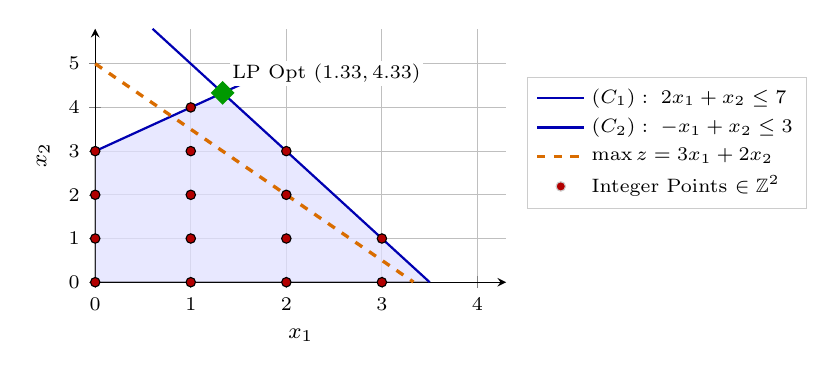
\begin{tikzpicture}
    \begin{axis}[
      width=6.8cm,
      height=4.8cm,
      axis lines=left,
      xmin=0, xmax=4.3,
      ymin=0, ymax=5.8,
      xlabel={$x_1$},
      ylabel={$x_2$},
      xtick={0,1,2,3,4},
      ytick={0,1,2,3,4,5},
      tick label style={font=\scriptsize},
      label style={font=\footnotesize},
      grid=major,
      clip=false,
      legend style={at={(1.05,0.55)}, anchor=west, draw=gray!40, fill=white, font=\scriptsize, cells={anchor=west}}
    ]

      % Feasible Region polygon
      % Vertices: (0,0), (3.5,0), (4/3,13/3), (0,3)
      \addplot[feasible area, forget plot] coordinates {(0,0) (3.5,0) (1.333,4.333) (0,3)} \closedcycle;

      % Constraints
      \addplot[constraint line, domain=0.6:3.5] {7 - 2*x};
      \addlegendentry{$(C_1):\; 2x_1 + x_2 \le 7$}
      \addplot[constraint line, domain=0:1.65] {3 + x};
      \addlegendentry{$(C_2):\; -x_1 + x_2 \le 3$}

      % Objective function level set (z=10 => x2 = 5 - 1.5 x1)
      \addplot[objective line, domain=0:3.33] {5 - 1.5*x};
      \addlegendentry{$\max z = 3x_1 + 2x_2$}

      % Integer points inside region (including (1,4))
      \addplot[integer point] coordinates {
        (0,0) (1,0) (2,0) (3,0)
        (0,1) (1,1) (2,1) (3,1)
        (0,2) (1,2) (2,2)
        (0,3) (1,3) (2,3)
        (1,4)
      };
      \addlegendentry{Integer Points $\in \mathbb{Z}^2$}

      % LP Optimum (intersection C1 & C2) = (4/3, 13/3)
      \coordinate (LP_Opt) at (axis cs:1.333, 4.333);
      \node[lp optimal, label={[font=\scriptsize, fill=white, inner sep=1pt, anchor=south west]above right:LP Opt $(1.33, 4.33)$}] at (LP_Opt) {};

    \end{axis}
  \end{tikzpicture}

  \vspace{-0.3em}
  \footnotesize
  \begin{itemize}
    \item The shaded region is the continuous LP feasible space; red dots ($\bullet$) are the 15 integer-feasible solutions.
    \item \textbf{LP Optimum ($\Diamond$):} $(x_1^*,x_2^*)=(4/3,13/3)$ with $z^* = 12.67$.
  \end{itemize}
\end{frame}

% ----------------------------------------------------------------------
% SLIDE 5: The Failure of Rounding
% ----------------------------------------------------------------------
\begin{frame}{Why the LP Solution is Not Enough}
  \footnotesize
  The common mistake is to simply round the fractional LP solution to the nearest integer point.

  \vspace{0.2em}
  \begin{columns}[T]
    \begin{column}{0.48\textwidth}
      \begin{itemize}
        \item \textbf{LP Optimum:} $(4/3,13/3)\approx(1.33,4.33)$, $z\approx12.67$.
        \item \textbf{Nearest Integer Points (Rounding):}
        \begin{itemize}
          \item Down-round: $(1,4)$, $z=3(1)+2(4)=\mathbf{11}$ (feasible).
          \item Up-round: $(2,5)$ (infeasible: $2(2)+5=9 \not\le 7$).
          \item Mixed: $(2,4)$ (infeasible: $2(2)+4=8 \not\le 7$).
        \end{itemize}
      \end{itemize}
      \vspace{0.3em}
      \alert{Rounding can be feasible but sub-optimal.}

      \vspace{0.3em}
      \textbf{True ILP Optimum:}
      \begin{itemize}
        \item Search the integer lattice points.
        \item Optimum at $\star$: $(2,3)$, $z=3(2)+2(3)=\mathbf{12}$.
      \end{itemize}
    \end{column}
    \begin{column}{0.50\textwidth}
      \centering
      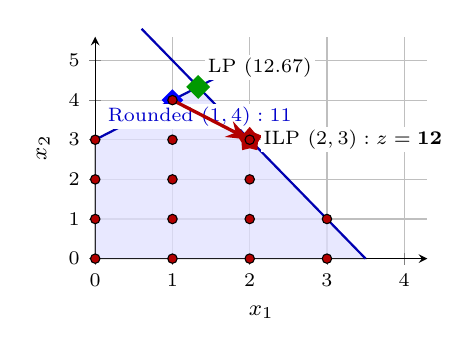
\begin{tikzpicture}
        \begin{axis}[
          width=5.8cm,
          height=4.4cm,
          axis lines=left,
          xmin=0, xmax=4.3,
          ymin=0, ymax=5.6,
          xlabel={$x_1$},
          ylabel={$x_2$},
          xtick={0,1,2,3,4},
          ytick={0,1,2,3,4,5},
          tick label style={font=\scriptsize},
          label style={font=\footnotesize},
          grid=major,
          clip=false
        ]
          \addplot[feasible area] coordinates {(0,0) (3.5,0) (1.333,4.333) (0,3)} \closedcycle;

          \addplot[constraint line, domain=0.6:3.5] {7 - 2*x};
          \addplot[constraint line, domain=0:1.65] {3 + x};

          \addplot[integer point] coordinates {
            (0,0) (1,0) (2,0) (3,0)
            (0,1) (1,1) (2,1) (3,1)
            (0,2) (1,2) (2,2)
            (0,3) (1,3) (2,3)
            (1,4)
          };

          % LP Optimum
          \coordinate (LP_Opt) at (axis cs:1.333, 4.333);
          \node[lp optimal, label={[font=\scriptsize, fill=white, inner sep=1pt, anchor=south west]above right:LP $(12.67)$}] at (LP_Opt) {};

          % Rounded feasible (1,4)
          \coordinate (Rounded_Opt) at (axis cs:1,4);
          \node[diamond, fill=blue, inner sep=2pt] at (Rounded_Opt) {};
          \node[font=\scriptsize, blue!80!black, fill=white, inner sep=1pt, anchor=south west] at (axis cs:0.12, 3.25) {Rounded $(1,4): 11$};

          % True ILP Optimum (2,3)
          \coordinate (ILP_Opt) at (axis cs:2,3);
          \node[ilp optimal, label={[font=\scriptsize, fill=white, inner sep=1pt, anchor=west]right:ILP $(2,3): z=\mathbf{12}$}] at (ILP_Opt) {};

          \draw[-Stealth, very thick, red!70!black] (Rounded_Opt) -- (ILP_Opt);
        \end{axis}
      \end{tikzpicture}
    \end{column}
  \end{columns}

  \vspace{0.2em}
  \textbf{Conclusion:} The true ILP optimum ($\star$) beats the rounded LP point, requiring systematic ILP algorithms.
\end{frame}

% ----------------------------------------------------------------------
% SLIDE 5B: PuLP 4.0 Code for Simple Pure ILP
% ----------------------------------------------------------------------
\begin{frame}[fragile]{Solving the Pure ILP in Python (PuLP 4.0)}{Example 1: Continuous LP Relaxation vs. Pure ILP}
\begin{columns}[T]
\begin{column}{0.56\textwidth}
\begin{lstlisting}
import pulp

# 1. Initialize Pure ILP Model (PuLP 4.0 API)
prob = pulp.LpProblem("Simple_Pure_ILP", pulp.LpMaximize)

# 2. Integer Decision Variables: x1, x2 in Z_{>= 0}
x1 = prob.add_variable("x1", lowBound=0, cat=pulp.LpInteger)
x2 = prob.add_variable("x2", lowBound=0, cat=pulp.LpInteger)

# 3. Objective Function
prob += 3 * x1 + 2 * x2, "Total_Profit"

# 4. Resource Constraints
prob += 2 * x1 + x2 <= 7, "C1"
prob += -x1 + x2 <= 3, "C2"

# 5. Solve and inspect Result
res = prob.solve()
print(f"Status: {res.status.name}")
print(f"Optimal z* = {pulp.value(prob.objective):.2f}")
print(f"x1* = {x1.varValue}, x2* = {x2.varValue}")
\end{lstlisting}
\end{column}
\begin{column}{0.41\textwidth}
\begin{block}{Output Comparison}
\footnotesize
\begin{itemize}
  \item \textbf{LP Relaxation (\texttt{LpContinuous}):}
  \begin{itemize}
    \scriptsize
    \item $x_1^* = 1.33, \; x_2^* = 4.33$
    \item $z_{\text{LP}}^* = 12.67$
  \end{itemize}
  \item \textbf{Pure ILP (\texttt{LpInteger}):}
  \begin{itemize}
    \scriptsize
    \item \texttt{Status: Optimal}
    \item $x_1^* = 2.0, \; x_2^* = 3.0$
    \item $z_{\text{ILP}}^* = \mathbf{12.00}$
  \end{itemize}
\end{itemize}
\end{block}
\begin{alertblock}{PuLP 4.0 Tip}
\scriptsize
Use \texttt{prob.add\_variable(..., cat=pulp.LpInteger)} to enforce integrality and \texttt{res = prob.solve()} to capture the solution status object.
\end{alertblock}
\end{column}
\end{columns}
\end{frame}

% ----------------------------------------------------------------------
% SLIDE 6: Methods Summary (Commented Out)
% ----------------------------------------------------------------------
\begin{comment}
\begin{frame}{Solving Integer Linear Programs}{Bridging the Gap Between LP and ILP}
  Since simple rounding is unreliable, specialized methods guarantee optimal integer solutions.

  \begin{enumerate}
    \item \textbf{Cutting Plane Methods}
      \begin{itemize}
        \item Add inequalities (cuts) to the LP relaxation to remove fractional optima without excluding any integer-feasible points.
        \item Re-solve until an integer solution emerges.
      \end{itemize}

    \item \textbf{Branch-and-Bound (B\&B)}
      \begin{itemize}
        \item Solve the LP relaxation.
        \item If fractional, \textbf{branch} (e.g., $x_1 \le \lfloor x_1^* \rfloor$ vs. $x_1 \ge \lceil x_1^* \rceil$).
        \item Use \textbf{bounds} to prune nodes that cannot improve the incumbent integer solution.
      \end{itemize}
  \end{enumerate}
\end{frame}
\end{comment}

\section{Branch and Bound Method}
\begin{frame}\sectionpage\end{frame}

% ----------------------------------------------------------------------
% SLIDE A: Branch-and-Bound — Idea
% ----------------------------------------------------------------------
\begin{frame}{Branch-and-Bound (B\&B): The Idea}
\vspace{-0.4em}
\begin{columns}[T]
  \begin{column}{0.52\textwidth}
    \begin{block}{Why B\&B?}
      \footnotesize
      \begin{itemize}
        \item LP relaxation is fast but may yield fractional values.
        \item ILP requires integrality; naive rounding can be suboptimal or infeasible.
      \end{itemize}
    \end{block}
    \vspace{-0.5em}
    \begin{block}{Core Mechanics}
      \footnotesize
      \begin{enumerate}
        \item \textbf{Relax} integrality and solve the LP $\Rightarrow$ upper bound (UB).
        \item \textbf{Branch} on a fractional variable ($x_i \le \lfloor x_i^*\rfloor$ vs. $x_i \ge \lceil x_i^*\rceil$).
        \item \textbf{Bound:} prune subproblems whose LP bound $\le$ best known integer solution (incumbent), or infeasible.
        \item Continue until all nodes are pruned or integer.
      \end{enumerate}
    \end{block}
    \vspace{-0.2em}
    \footnotesize
    \alert{Goal:} Prove optimality by excluding all non-promising regions.
  \end{column}
  \begin{column}{0.45\textwidth}
    \begin{block}{Our ILP (Same as Before)}
      \footnotesize
      \[
        \max z = 3x_1 + 2x_2
      \]
      \vspace{-0.8em}
      \[
        \begin{aligned}
          2x_1 + x_2 &\le 7,\\
          -x_1 + x_2 &\le 3,\\
          x_1, x_2 &\ge 0, \quad x_1,x_2 \in \mathbb{Z}.
        \end{aligned}
      \]
      \textbf{Root LP Relaxation Optimum:}\\
      $(x_1^*,x_2^*)=\left(\tfrac{4}{3},\tfrac{13}{3}\right), \quad z^* \approx 12.67$ (fractional).
    \end{block}
  \end{column}
\end{columns}
\end{frame}

% ----------------------------------------------------------------------
% SLIDE B: Branch on x2 at the root
% ----------------------------------------------------------------------
\begin{frame}{B\&B Step 1: Branch on the Fractional Variable}
  \centering
  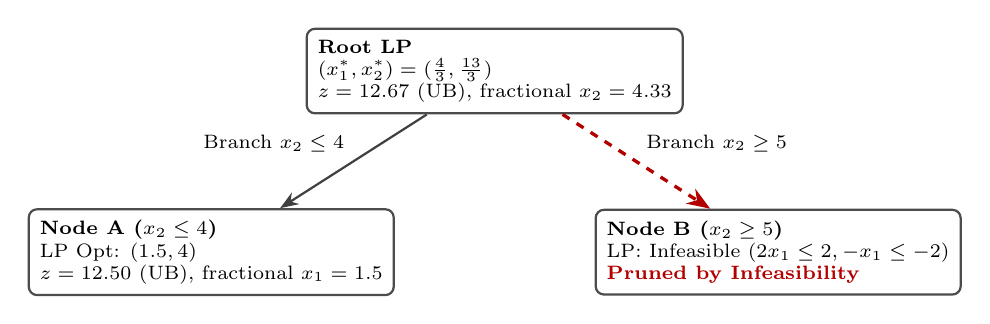
\begin{tikzpicture}[on grid, node distance=2.3cm and 3.6cm]
    \node[bnb node] (root) {\textbf{Root LP}\\
      $(x_1^*,x_2^*) = (\tfrac{4}{3},\tfrac{13}{3})$\\
      $z = 12.67$ (UB), fractional $x_2 = 4.33$
    };
    \node[bnb node, below left=of root] (A) {\textbf{Node A ($x_2 \le 4$)}\\
      LP Opt: $(1.5, 4)$\\
      $z = 12.50$ (UB), fractional $x_1 = 1.5$
    };
    \node[bnb node, below right=of root] (B) {\textbf{Node B ($x_2 \ge 5$)}\\
      LP: Infeasible ($2x_1 \le 2, -x_1 \le -2$)\\
      \textcolor{red!70!black}{\textbf{Pruned by Infeasibility}}
    };

    \draw[bnb edge] (root) -- node[above left, font=\scriptsize, pos=0.5, inner sep=3pt] {Branch $x_2 \le 4$} (A);
    \draw[bnb edge, bnb no] (root) -- node[above right, font=\scriptsize, pos=0.5, inner sep=3pt] {Branch $x_2 \ge 5$} (B);
  \end{tikzpicture}
\end{frame}

% ----------------------------------------------------------------------
% SLIDE C2: Branch Node A on x1 — tree & summary
% ----------------------------------------------------------------------
\begin{frame}{B\&B Step 2: Complete Search Tree and Bounds}
  \centering
  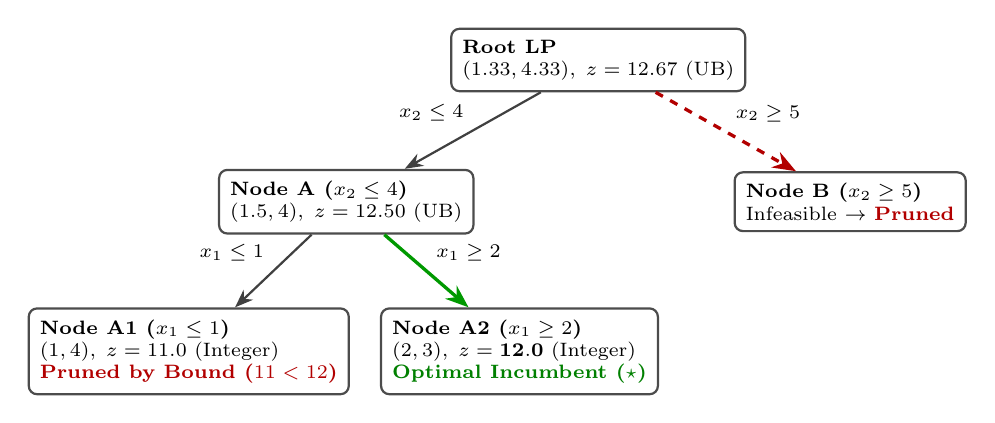
\begin{tikzpicture}[on grid]
    \node[bnb node] (root) at (0,0) {\textbf{Root LP}\\ $(1.33, 4.33),\; z = 12.67$ (UB)};
    \node[bnb node] (A) at (-3.2,-1.8) {\textbf{Node A ($x_2 \le 4$)}\\ $(1.5, 4),\; z = 12.50$ (UB)};
    \node[bnb node] (B) at (3.2,-1.8) {\textbf{Node B ($x_2 \ge 5$)}\\ Infeasible $\rightarrow$ \textcolor{red!70!black}{\textbf{Pruned}}};

    \draw[bnb edge] (root) -- node[above left, font=\scriptsize, inner sep=3pt] {$x_2 \le 4$} (A);
    \draw[bnb edge, bnb no] (root) -- node[above right, font=\scriptsize, inner sep=3pt] {$x_2 \ge 5$} (B);

    \node[bnb node] (A1) at (-5.2,-3.7) {\textbf{Node A1 ($x_1 \le 1$)}\\ $(1, 4),\; z = 11.0$ (Integer)\\ \textcolor{red!70!black}{\textbf{Pruned by Bound ($11 < 12$)}}};
    \node[bnb node] (A2) at (-1.0,-3.7) {\textbf{Node A2 ($x_1 \ge 2$)}\\ $(2, 3),\; z = \mathbf{12.0}$ (Integer)\\ \textcolor{green!50!black}{\textbf{Optimal Incumbent ($\star$)}}};

    \draw[bnb edge] (A) -- node[above left, font=\scriptsize, inner sep=3pt] {$x_1 \le 1$} (A1);
    \draw[bnb edge, bnb yes] (A) -- node[above right, font=\scriptsize, inner sep=3pt] {$x_1 \ge 2$} (A2);
  \end{tikzpicture}
\end{frame}


% ----------------------------------------------------------------------
% SECTION: The 0-1 Knapsack Problem
% ----------------------------------------------------------------------
\section{The 0-1 Knapsack Problem}
\begin{frame}\sectionpage\end{frame}

\begin{frame}{Problem Definition: The 0-1 Knapsack}{What is the 0-1 Knapsack Problem?}
    \begin{block}{The Classic Analogy}
        Imagine you have a knapsack (or bag) with a limited weight capacity, $W$.
    \end{block}

    \begin{columns}[T]
        \begin{column}{0.50\textwidth}
            \begin{itemize}
                \item You are presented with $n$ different items.
                \item Each item $i$ has:
                \begin{itemize}
                    \item A \textbf{value}, $v_i$
                    \item A \textbf{weight}, $w_i$
                \end{itemize}
                \item You must make a binary (``0-1'') decision for each item:
                \begin{itemize}
                    \item Either you \textbf{take} the item ($x_i = 1$)
                    \item Or you \textbf{leave} the item ($x_i = 0$)
                \end{itemize}
                \item You cannot take fractions of items.
            \end{itemize}
        \end{column}
        \begin{column}{0.46\textwidth}
            \begin{alertblock}{The Goal}
                \centering
                Choose the combination of items that \textbf{maximizes the total value} in your knapsack...
                \vspace{0.8em}

                ...without \textbf{exceeding the total weight capacity} $W$.
            \end{alertblock}
        \end{column}
    \end{columns}
\end{frame}

% ----------------------------------------------------------------------
% SLIDE 3: A Simple Example
% ----------------------------------------------------------------------
\begin{frame}{A Simple Knapsack Example}{Which Items Should We Take?}
    \footnotesize
    Let's define a specific problem:

    \begin{block}{Knapsack Capacity}
        \centering
        Maximum Weight ($W$) = \textbf{10 kg}
    \end{block}

    \begin{block}{Available Items ($n=4$)}
        \centering
        \begin{tabular}{cccc}
        \toprule
        \textbf{Item ($i$)} & \textbf{Name} & \textbf{Value ($v_i$)} & \textbf{Weight ($w_i$)} \\
        \midrule
        1 & Laptop & \$40 & 4 kg \\
        2 & Gold & \$50 & 3 kg \\
        3 & Silver & \$30 & 6 kg \\
        4 & Books & \$10 & 5 kg \\
        \bottomrule
        \end{tabular}
    \end{block}

    \begin{alertblock}{The Question}
        \centering
        How do we formally model the decision to maximize total value without exceeding 10 kg?
    \end{alertblock}
\end{frame}

% ----------------------------------------------------------------------
% SLIDE 4: ILP Formulation
% ----------------------------------------------------------------------
\begin{frame}{ILP Formulation}{Translating the Problem into Math}
    We can model this problem using Binary Integer Linear Programming:

    \begin{columns}[T]
        \begin{column}{0.48\textwidth}
            \begin{block}{1. Decision Variables}
                \begin{itemize}
                    \item For each item $i$, define a binary variable $x_i \in \{0, 1\}$:
                    \item $x_i = 1$ if we \textbf{take} item $i$
                    \item $x_i = 0$ if we \textbf{leave} item $i$
                \end{itemize}
                \vspace{0.4em}
                \centering
                \footnotesize $x_1$: Laptop,\; $x_2$: Gold,\; $x_3$: Silver,\; $x_4$: Books
            \end{block}
        \end{column}
        \begin{column}{0.48\textwidth}
            \begin{block}{2. Objective Function (Maximize Value)}
                Maximize the total value of selected items:
                \[ \max z = \sum_{i=1}^{4} v_i x_i = 40x_1 + 50x_2 + 30x_3 + 10x_4 \]
            \end{block}
            \begin{block}{3. Constraint (Weight Capacity)}
                Total weight cannot exceed $W = 10$:
                \[ 4x_1 + 3x_2 + 6x_3 + 5x_4 \le 10 \]
            \end{block}
        \end{column}
    \end{columns}
\end{frame}

% ----------------------------------------------------------------------
% SLIDE 5: Greedy Solution (Placed BEFORE Solution & Conclusion)
% ----------------------------------------------------------------------
\begin{frame}{Greedy Solution}{Evaluating the Value-to-Weight Ratio Heuristic}
    \begin{block}{How Does a ``Greedy'' Heuristic Work?}
        \begin{itemize}
            \item Rank items by highest ``bang for the buck'' (value per kg, $v_i / w_i$):
            \begin{itemize}
                \item \textbf{1. Gold:} $\$50 / 3\text{ kg} = \$16.67/\text{kg}$
                \item \textbf{2. Laptop:} $\$40 / 4\text{ kg} = \$10.00/\text{kg}$
                \item \textbf{3. Silver:} $\$30 / 6\text{ kg} = \$5.00/\text{kg}$
                \item \textbf{4. Books:} $\$10 / 5\text{ kg} = \$2.00/\text{kg}$
            \end{itemize}
            \item \textbf{Greedy Step 1:} Take Gold ($x_2=1$). \textit{Value = \$50, Weight = 3 kg (7 kg left).}
            \item \textbf{Greedy Step 2:} Take Laptop ($x_1=1$). \textit{Value = $\$50+\$40=\mathbf{\$90}$, Weight = $3+4=7$ kg (3 kg left).}
            \item Neither Silver (6 kg) nor Books (5 kg) fit in the remaining 3 kg.
            \item \textbf{Greedy Candidate:} $\{\text{Laptop, Gold}\}$ with $z = \$90$.
        \end{itemize}
    \end{block}
\end{frame}

% ----------------------------------------------------------------------
% SLIDE 6: Solution & Conclusion
% ----------------------------------------------------------------------
\begin{frame}{Solution \& Conclusion}{Solving the 0-1 Knapsack ILP}
    \footnotesize
    \begin{block}{The Complete 0-1 Knapsack ILP Model}
        \vspace{-0.6em}
        \begin{align*}
            \max \quad z = & \; 40x_1 + 50x_2 + 30x_3 + 10x_4 \\
            \text{s.t.} \quad & \; 4x_1 + 3x_2 + 6x_3 + 5x_4 \le 10 \\
            & \; x_1, x_2, x_3, x_4 \in \{0, 1\}
        \end{align*}
    \end{block}
    \begin{alertblock}{Optimal ILP Solution}
        \begin{itemize}
            \item Solving the exact ILP confirms that the greedy candidate \textbf{is} optimal in this instance:
            \item $x_1^*=1, \; x_2^*=1, \; x_3^*=0, \; x_4^*=0$
            \item Optimal Value: $z^* = 40(1) + 50(1) + 0 + 0 = \mathbf{\$90}$
            \item Total Weight: $w = 4(1) + 3(1) = 7\text{ kg} \le 10\text{ kg}$
            \item \textit{Comparison:} $\{\text{Gold, Silver}\}$ uses more capacity ($w=9\text{ kg}$) but yields lower value ($z=\$80$).
        \end{itemize}
    \end{alertblock}
\end{frame}

\begin{frame}{Observations}{When Greedy Fails vs. Exact ILP}
    \begin{block}{Reflecting on the Knapsack Solution}
        \begin{itemize}
            \item Greedy heuristics often \textbf{fail} for 0-1 Knapsack problems (even though it happened to match the optimum here).
            \item \textit{Counterexample:} If Silver weighed 7 kg with value \$45 ($v_3/w_3 = \$6.43/\text{kg}$), Greedy would still pick $\{\text{Gold, Laptop}\}$ ($z=\$90, w=7$), whereas $\{\text{Gold, Silver}\}$ would achieve $z=\$95, w=10$!
            \item The ILP formulation guarantees the true global optimum.
            \item For large $n$, 0-1 Knapsack is $\mathcal{NP}$-hard and solved via Branch-and-Bound or Dynamic Programming.
        \end{itemize}
    \end{block}
\end{frame}

% ----------------------------------------------------------------------
% SLIDE: PuLP 4.0 Code for 0-1 Knapsack
% ----------------------------------------------------------------------
\begin{frame}[fragile]{Solving the 0-1 Knapsack in Python (PuLP 4.0)}{Example 2: Binary Decision Variables with \texttt{add\_variable\_dicts}}
\begin{columns}[T]
\begin{column}{0.58\textwidth}
\begin{lstlisting}
import pulp

items = ["Laptop", "Gold", "Silver", "Books"]
val = {"Laptop": 40, "Gold": 50, "Silver": 30, "Books": 10}
wt  = {"Laptop": 4,  "Gold": 3,  "Silver": 6,  "Books": 5}

prob = pulp.LpProblem("Knapsack_0_1", pulp.LpMaximize)

# Binary variables x[i] in {0, 1} using PuLP 4.0 API
x = prob.add_variable_dicts("x", items, cat=pulp.LpBinary)

# Objective & Weight Capacity Constraint
prob += pulp.lpSum(val[i] * x[i] for i in items), "Total_Value"
prob += pulp.lpSum(wt[i] * x[i] for i in items) <= 10, "Max_Weight"

res = prob.solve()
z_opt = pulp.value(prob.objective)
print(f"Status: {res.status.name}, Optimal Value = ${z_opt:.0f}")
for i in items:
    if x[i].varValue > 0.5:
        print(f"  Take {i}: weight={wt[i]} kg, value=${val[i]}")
\end{lstlisting}
\end{column}
\begin{column}{0.39\textwidth}
\begin{block}{Console Output}
\footnotesize
\texttt{Status: Optimal}\\
\texttt{Optimal Value = \$90}\\
\texttt{Take Laptop: weight=4 kg, value=\$40}\\
\texttt{Take Gold: weight=3 kg, value=\$50}
\end{block}
\begin{alertblock}{Key Takeaway}
\scriptsize
\texttt{cat=pulp.LpBinary} restricts each variable to $\{0, 1\}$. Using \texttt{prob.add\_variable\_dicts} scales cleanly to hundreds of items.
\end{alertblock}
\end{column}
\end{columns}
\end{frame}


\section{The 0-1 Knapsack Problem: Logical Constraints}
\begin{frame}\sectionpage\end{frame}

% ----------------------------------------------------------------------
% SLIDE 2: Base Model (Standard Knapsack)
% ----------------------------------------------------------------------
\begin{frame}{The Base Knapsack Problem (KP)}{Standard Binary Integer Programming Model}
    \begin{columns}[T]
        \begin{column}{0.48\textwidth}
            \begin{block}{Decision Variables}
                For each item $i$, let $x_i$ be a \textbf{binary decision variable}:
                \[ x_i = \begin{cases}
                    1 & \text{if item } i \text{ is selected} \\
                    0 & \text{otherwise}
                \end{cases} \]
            \end{block}

            \begin{block}{Model Notation}
                \begin{itemize}
                    \item $v_i$: Value of item $i$
                    \item $w_i$: Weight of item $i$
                    \item $C$: Capacity of the knapsack
                \end{itemize}
            \end{block}
        \end{column}
        \begin{column}{0.48\textwidth}
            \begin{alertblock}{The Standard KP Model}
                \[ \max \sum_{i \in I} v_i x_i \]
                \[ \text{s.t.} \quad \sum_{i \in I} w_i x_i \le C \]
                \[ \quad x_i \in \{0, 1\}, \quad \forall i \in I \]
            \end{alertblock}

            \begin{itemize}
                \item Next, we add \textbf{logical conditions} (implications, requirements, conflicts) using linear inequalities.
            \end{itemize}
        \end{column}
    \end{columns}
\end{frame}

% ----------------------------------------------------------------------
% SLIDE 3: Complication 1: Conditional Inclusion (Implication)
% ----------------------------------------------------------------------
\begin{frame}{Complication 1: Conditional Inclusion}{Rule: If Item 1 is Taken, Then Item 2 Must Be Taken}
    \begin{constraintblock}{$x_1 = 1 \implies x_2 = 1$}
        This is a logical implication constraint. If the premise ($x_1=1$) is true, the conclusion ($x_2=1$) must also be true.
    \end{constraintblock}

    \begin{columns}[T]
        \begin{column}{0.50\textwidth}
            \begin{alertblock}{Test Cases (All Combinations)}
            \footnotesize
                \begin{itemize}
                    \item $x_1=1, x_2=0 \implies 1-0 = 1 \not\le 0$ (\textbf{Violates} $\rightarrow$ \alert{Excluded})
                    \item $x_1=1, x_2=1 \implies 1-1 = 0 \le 0$ (\textbf{Satisfies} $\rightarrow$ Feasible)
                    \item $x_1=0, x_2=0 \implies 0-0 = 0 \le 0$ (\textbf{Satisfies} $\rightarrow$ Feasible)
                    \item $x_1=0, x_2=1 \implies 0-1 = -1 \le 0$ (\textbf{Satisfies} $\rightarrow$ Feasible)
                \end{itemize}
            \end{alertblock}
        \end{column}
        \begin{column}{0.46\textwidth}
            \begin{block}{The MILP Constraint}
                \centering $\mathbf{x_1 - x_2 \le 0} \quad (\text{or } \mathbf{x_1 \le x_2})$
            \end{block}
            \centering
            \footnotesize \textbf{Visualization of Feasible Combinations}\\[2pt]
            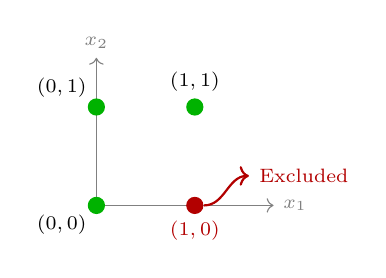
\begin{tikzpicture}[scale=1.25, every node/.style={font=\scriptsize}]
                \draw[->, gray] (0,0) -- (1.8,0) node[right] {$x_1$};
                \draw[->, gray] (0,0) -- (0,1.5) node[above] {$x_2$};

                % Feasible Points (Green)
                \node[circle, fill=green!70!black, inner sep=2.2pt] (A) at (0, 0) {};
                \node[circle, fill=green!70!black, inner sep=2.2pt] (B) at (0, 1) {};
                \node[circle, fill=green!70!black, inner sep=2.2pt] (C) at (1, 1) {};

                % Infeasible Point (Red)
                \node[circle, fill=red!70!black, inner sep=2.2pt] (D) at (1, 0) {};

                % Labels
                \node[below left] at (A) {$(0,0)$};
                \node[above left] at (B) {$(0,1)$};
                \node[above=2pt] at (C) {$(1,1)$};
                \node[below=2pt, red!70!black] at (D) {$(1,0)$};

                \draw[red!70!black, thick, ->] (D) to[out=0, in=180] (1.55, 0.3) node[right] {Excluded};
            \end{tikzpicture}
        \end{column}
    \end{columns}
\end{frame}

% ----------------------------------------------------------------------
% SLIDE 4: Complication 2: Mandatory Inclusion
% ----------------------------------------------------------------------
\begin{frame}{Complication 2: Mandatory Inclusion}{Rule: Item 1 Must Be Taken}
    \vspace{-0.2em}
    \begin{constraintblock}{$x_1 = 1$}
        This is the simplest form of logical constraint, forcing a specific binary decision to be true regardless of other factors (as long as capacity allows).
    \end{constraintblock}
    \vspace{-0.2em}
    \begin{columns}[T]
        \begin{column}{0.50\textwidth}
            \begin{alertblock}{Impact on the Model}
            \footnotesize
                \begin{itemize}
                    \item All feasible solutions must now include Item 1.
                    \item The objective and capacity constraints effectively become:
                    \[ \max \left(v_1 + \sum_{i \in I \setminus \{1\}} v_i x_i\right) \]
                    \[ \text{s.t.} \quad w_1 + \sum_{i \in I \setminus \{1\}} w_i x_i \le C \]
                \end{itemize}
            \end{alertblock}
        \end{column}
        \begin{column}{0.46\textwidth}
            \begin{block}{The MILP Constraint}
                \centering $\mathbf{x_1 = 1}$
            \end{block}
            \centering
            \footnotesize \textbf{Visualization: Forcing $x_1=1$}\\[2pt]
            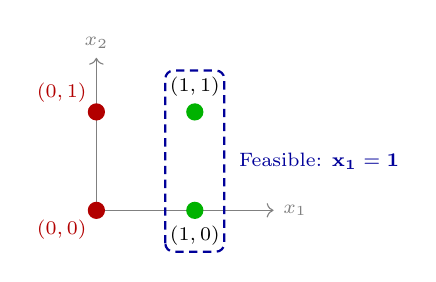
\begin{tikzpicture}[scale=1.25, every node/.style={font=\scriptsize}]
                \draw[->, gray] (0,0) -- (1.8,0) node[right] {$x_1$};
                \draw[->, gray] (0,0) -- (0,1.55) node[above] {$x_2$};

                % Infeasible Points (Red)
                \node[circle, fill=red!70!black, inner sep=2.2pt] (A) at (0, 0) {};
                \node[circle, fill=red!70!black, inner sep=2.2pt] (B) at (0, 1) {};

                % Feasible Points (Green)
                \node[circle, fill=green!70!black, inner sep=2.2pt] (C) at (1, 1) {};
                \node[circle, fill=green!70!black, inner sep=2.2pt] (D) at (1, 0) {};

                % Labels
                \node[below left, red!70!black] at (A) {$(0,0)$};
                \node[above left, red!70!black] at (B) {$(0,1)$};
                \node[above=2pt] at (C) {$(1,1)$};
                \node[below=2pt] at (D) {$(1,0)$};

                \draw[thick, blue!60!black, densely dashed, rounded corners=3pt] (0.70, -0.42) rectangle (1.30, 1.42);
                \node[blue!60!black, right] at (1.35, 0.5) {Feasible: $\mathbf{x_1 = 1}$};
            \end{tikzpicture}
        \end{column}
    \end{columns}
\end{frame}

% ----------------------------------------------------------------------
% SLIDE 5: Complication 3: Mutual Exclusion
% ----------------------------------------------------------------------
\begin{frame}{Complication 3: Mutual Exclusion (Prohibition)}{Rule: If Item 1 is Taken, Then Item 2 Cannot Be Taken}
    \begin{constraintblock}{$x_1 = 1 \implies x_2 = 0$}
        This relationship is symmetric for binary variables. If we take Item 1, we exclude Item 2, and if we take Item 2, we exclude Item 1. This is known as a \textbf{Mutual Exclusion} constraint.
    \end{constraintblock}

    \begin{columns}[T]
        \begin{column}{0.50\textwidth}
            \begin{alertblock}{Test Cases (All Combinations)}
            \footnotesize
                \begin{itemize}
                    \item $x_1=1, x_2=1 \implies 1+1 = 2 \not\le 1$ (\textbf{Violates} $\rightarrow$ \alert{Excluded})
                    \item $x_1=1, x_2=0 \implies 1+0 = 1 \le 1$ (\textbf{Satisfies} $\rightarrow$ Feasible)
                    \item $x_1=0, x_2=1 \implies 0+1 = 1 \le 1$ (\textbf{Satisfies} $\rightarrow$ Feasible)
                    \item $x_1=0, x_2=0 \implies 0+0 = 0 \le 1$ (\textbf{Satisfies} $\rightarrow$ Feasible)
                \end{itemize}
            \end{alertblock}
        \end{column}
        \begin{column}{0.46\textwidth}
            \begin{block}{The MILP Constraint}
                \centering $\mathbf{x_1 + x_2 \le 1}$
            \end{block}
            \centering
            \footnotesize \textbf{Visualization of Feasible Combinations}\\[2pt]
            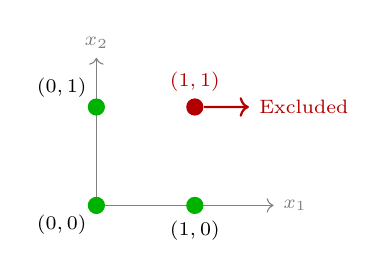
\begin{tikzpicture}[scale=1.25, every node/.style={font=\scriptsize}]
                \draw[->, gray] (0,0) -- (1.8,0) node[right] {$x_1$};
                \draw[->, gray] (0,0) -- (0,1.5) node[above] {$x_2$};

                % Feasible Points (Green)
                \node[circle, fill=green!70!black, inner sep=2.2pt] (A) at (0, 0) {};
                \node[circle, fill=green!70!black, inner sep=2.2pt] (B) at (0, 1) {};
                \node[circle, fill=green!70!black, inner sep=2.2pt] (D) at (1, 0) {};

                % Infeasible Point (Red)
                \node[circle, fill=red!70!black, inner sep=2.2pt] (C) at (1, 1) {};

                % Labels
                \node[below left] at (A) {$(0,0)$};
                \node[above left] at (B) {$(0,1)$};
                \node[below=2pt] at (D) {$(1,0)$};
                \node[above=2pt, red!70!black] at (C) {$(1,1)$};

                \draw[red!70!black, thick, ->] (C) to[out=0, in=180] (1.55, 1.0) node[right] {Excluded};
            \end{tikzpicture}
        \end{column}
    \end{columns}
\end{frame}

% ----------------------------------------------------------------------
% SLIDE 6: Complication 4: Exclusive OR
% ----------------------------------------------------------------------
\begin{frame}{Complication 4: Exclusive OR (XOR)}{Rule: Either Item 1 OR Item 2 Must Be Taken (But Not Both)}
    \vspace{-0.2em}
    \begin{constraintblock}{$(x_1 = 1 \text{ XOR } x_2 = 1)$}
        This constraint requires an exact choice of one item from the pair: \textbf{at least one} must be chosen ($x_1 + x_2 \ge 1$), and \textbf{at most one} can be chosen ($x_1 + x_2 \le 1$).
    \end{constraintblock}
    \vspace{-0.2em}
    \begin{columns}[T]
        \begin{column}{0.50\textwidth}
            \begin{alertblock}{Test Cases (All Combinations)}
                \footnotesize
                \begin{itemize}
                    \item $x_1=1, x_2=1 \implies 1+1 = 2 \ne 1$ (\alert{Excluded})
                    \item $x_1=1, x_2=0 \implies 1+0 = 1$ (\textbf{Satisfies} $\rightarrow$ Feasible)
                    \item $x_1=0, x_2=1 \implies 0+1 = 1$ (\textbf{Satisfies} $\rightarrow$ Feasible)
                    \item $x_1=0, x_2=0 \implies 0+0 = 0 \ne 1$ (\alert{Excluded})
                \end{itemize}
            \end{alertblock}
            \footnotesize
            \begin{itemize}
                \item Only the diagonal combinations $(\mathbf{1, 0})$ and $(\mathbf{0, 1})$ are allowed.
            \end{itemize}
        \end{column}
        \begin{column}{0.46\textwidth}
            \begin{block}{The MILP Constraint}
                \centering $\mathbf{x_1 + x_2 = 1}$
            \end{block}
            \centering
            \footnotesize \textbf{Visualization of Feasible Combinations}\\[2pt]
            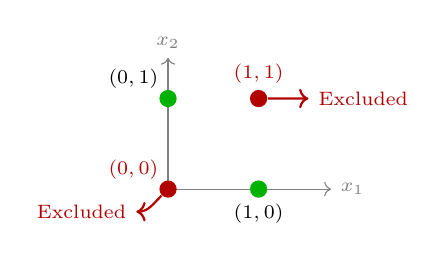
\begin{tikzpicture}[scale=1.15, every node/.style={font=\scriptsize}]
                \draw[->, gray] (0,0) -- (1.8,0) node[right] {$x_1$};
                \draw[->, gray] (0,0) -- (0,1.45) node[above] {$x_2$};

                % Infeasible Points (Red)
                \node[circle, fill=red!70!black, inner sep=2.2pt] (A) at (0, 0) {};
                \node[circle, fill=red!70!black, inner sep=2.2pt] (C) at (1, 1) {};

                % Feasible Points (Green)
                \node[circle, fill=green!70!black, inner sep=2.2pt] (B) at (0, 1) {};
                \node[circle, fill=green!70!black, inner sep=2.2pt] (D) at (1, 0) {};

                % Labels
                \node[above left, red!70!black] at (A) {$(0,0)$};
                \node[above left] at (B) {$(0,1)$};
                \node[below=2pt] at (D) {$(1,0)$};
                \node[above=2pt, red!70!black] at (C) {$(1,1)$};

                \draw[red!70!black, thick, ->] (A) to[out=225, in=0] (-0.35, -0.25) node[left] {Excluded};
                \draw[red!70!black, thick, ->] (C) to[out=0, in=180] (1.55, 1.0) node[right] {Excluded};
            \end{tikzpicture}
        \end{column}
    \end{columns}
\end{frame}

% ----------------------------------------------------------------------
% SLIDE: PuLP 4.0 Code for Knapsack with Logical Constraints
% ----------------------------------------------------------------------
\begin{frame}[fragile]{Knapsack with Logical Constraints in Python (PuLP 4.0)}{Example 3: Adding Mutual Exclusion and Implication Rules}
\begin{columns}[T]
\begin{column}{0.58\textwidth}
\begin{lstlisting}
import pulp

items = ["Laptop", "Gold", "Silver", "Books"]
val = {"Laptop": 40, "Gold": 50, "Silver": 30, "Books": 10}
wt  = {"Laptop": 4,  "Gold": 3,  "Silver": 6,  "Books": 5}

prob = pulp.LpProblem("Knapsack_Logical", pulp.LpMaximize)
x = prob.add_variable_dicts("x", items, cat=pulp.LpBinary)

prob += pulp.lpSum(val[i] * x[i] for i in items), "Total_Value"
prob += pulp.lpSum(wt[i] * x[i] for i in items) <= 10, "Max_Weight"

# Rule 1 (Mutual Exclusion): Cannot take both Laptop and Gold
prob += x["Laptop"] + x["Gold"] <= 1, "Mutually_Exclusive"

# Rule 2 (Implication): If Gold is taken, Books must be taken
prob += x["Gold"] - x["Books"] <= 0, "Gold_Implies_Books"

res = prob.solve()
z_opt = pulp.value(prob.objective)
print(f"Status: {res.status.name}, Optimal Value = ${z_opt:.0f}")
print("Selected:", [i for i in items if x[i].varValue > 0.5])
\end{lstlisting}
\end{column}
\begin{column}{0.39\textwidth}
\begin{block}{Impact of Logical Rules}
\footnotesize
\begin{itemize}
  \item \textbf{Option A (Take Gold):} Forces Books ($3+5=8$ kg), blocks Laptop; remaining 2 kg fits nothing $\Rightarrow z = 50 + 10 = \$60$.
  \item \textbf{Option B (Take Laptop + Silver):} $4+6=10$ kg $\le 10$ kg $\Rightarrow z = 40 + 30 = \mathbf{\$70}$.
\end{itemize}
\end{block}
\begin{alertblock}{Console Output}
\scriptsize
\texttt{Status: Optimal, Optimal Value = \$70}\\
\texttt{Selected: ['Laptop', 'Silver']}
\end{alertblock}
\end{column}
\end{columns}
\end{frame}


%------------------------------------------------------------------------------------------------------
\section{Modeling Fixed Setup Costs}
\begin{frame}\sectionpage\end{frame}

% ----------------------------------------------------------------------
% SLIDE 2: Problem Scenario
% ----------------------------------------------------------------------
\begin{frame}{Problem Scenario: Capacity and Production}{The Fixed Capacity Decision}
    A company manufactures two products, $x_1$ and $x_2$. They earn profits of \textbf{\$5 per unit of $x_1$} and \textbf{\$3 per unit of $x_2$}.

    \begin{block}{The Fixed Cost Element}
        Before any production can occur (i.e., if $x_1 > 0$ or $x_2 > 0$), a single facility must be activated at a \alert{\textbf{fixed cost of \$10}}.
    \end{block}

    \begin{columns}[T]
        \begin{column}{0.48\textwidth}
            \begin{block}{Constraints (Resources)}
                \begin{itemize}
                    \item $\mathbf{C_1}$ (Resource A): $x_1 + x_2 \le 10$
                    \item $\mathbf{C_2}$ (Resource B): $2x_1 + x_2 \le 16$
                    \item $\mathbf{C_3}$ (Resource C): $x_2 \le 7$
                \end{itemize}
            \end{block}
        \end{column}
        \begin{column}{0.48\textwidth}
            \begin{block}{Decision Required}
                The final solution must choose between:
                \begin{enumerate}
                    \item \textbf{No Production ($y=0$):} Total Profit $Z=0$.
                    \item \textbf{Production ($y=1$):} Total Profit $= (\text{Gross Profit}) - \$10$.
                \end{enumerate}
            \end{block}
        \end{column}
    \end{columns}
\end{frame}

% ----------------------------------------------------------------------
% SLIDE 3: The Continuous Relaxation (Ignoring Fixed Cost)
% ----------------------------------------------------------------------
\begin{frame}{Step 1: The Continuous LP Relaxation}{Solving for Maximum Gross Profit}
    We first maximize the gross profit $\mathbf{Z_{\text{gross}} = 5x_1 + 3x_2}$ while ignoring the fixed cost of \$10.

    \begin{columns}[T]
        \begin{column}{0.43\textwidth}
            \begin{block}{LP Formulation}
                \[ \max Z_{\text{gross}} = 5x_1 + 3x_2 \]
                \[\begin{aligned}
                    \text{s.t.} \quad &x_1 + x_2 \le 10 & (C_1)\\
                    &2x_1 + x_2 \le 16 & (C_2)\\
                    &\qquad x_2 \le 7 & (C_3)\\
                    &x_1, x_2 \ge 0
                \end{aligned}\]
            \end{block}
        \end{column}
        \begin{column}{0.54\textwidth}
            \centering
            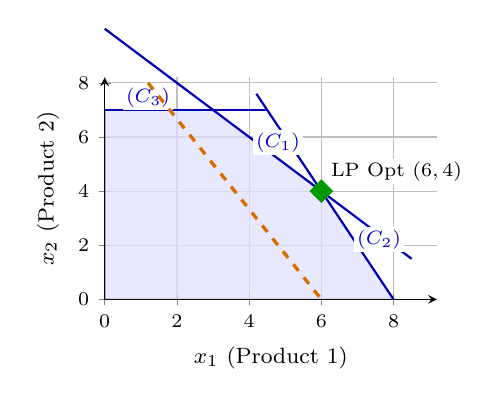
\begin{tikzpicture}
                \begin{axis}[
                    width=5.8cm,
                    height=4.4cm,
                    axis lines=left,
                    xmin=0, xmax=9.2, ymin=0, ymax=8.2,
                    xlabel={$x_1$ (Product 1)}, ylabel={$x_2$ (Product 2)},
                    xtick={0, 2, 4, 6, 8}, ytick={0, 2, 4, 6, 8},
                    tick label style={font=\scriptsize},
                    label style={font=\footnotesize},
                    grid=major, clip=false
                ]
                % Feasible Region (Vertices: (0,0), (8,0), (6,4), (3,7), (0,7))
                \addplot[feasible area] coordinates {(0, 0) (8, 0) (6, 4) (3, 7) (0, 7)} \closedcycle;

                % Constraint Lines
                \addplot[constraint line, domain=0:8.5] {10 - x};
                \addplot[constraint line, domain=4.2:8] {16 - 2*x};
                \draw[constraint line] (axis cs:0, 7) -- (axis cs:4.5, 7);
                \node[font=\scriptsize, blue!80!black, fill=white, inner sep=1pt] at (axis cs:4.8, 5.8) {$(C_1)$};
                \node[font=\scriptsize, blue!80!black, fill=white, inner sep=1pt] at (axis cs:7.6, 2.2) {$(C_2)$};
                \node[font=\scriptsize, blue!80!black, fill=white, inner sep=1pt] at (axis cs:1.2, 7.45) {$(C_3)$};

                % LP Optimal Solution (6, 4)
                \coordinate (LP_Opt) at (axis cs:6, 4);
                \node[lp optimal, label={[font=\scriptsize, fill=white, inner sep=1pt, anchor=south west]above right:\alert{LP Opt $(6, 4)$}}] at (LP_Opt) {};

                % Objective Line (Z_gross = 30 => x2 = 10 - (5/3)*x1)
                \addplot[objective line, domain=1.2:6] {10 - (5/3)*x};
                \end{axis}
            \end{tikzpicture}
        \end{column}
    \end{columns}
\end{frame}

% ----------------------------------------------------------------------
% SLIDE 4: Result of LP Relaxation
% ----------------------------------------------------------------------
\begin{frame}{Result of LP Relaxation (Gross Profit)}{The Gross Optimal Solution}
    \begin{itemize}
        \item The optimal solution to the continuous Linear Program is found at the intersection of constraints $\mathbf{C_1}$ and $\mathbf{C_2}$:
        \[ \mathbf{C_1}: x_1 + x_2 = 10 \quad \big| \quad \mathbf{C_2}: 2x_1 + x_2 = 16 \]
        \item Solving these equations yields:
        \[ x_1^* = 6, \quad x_2^* = 4 \]
        \item \textbf{Maximum Gross Profit ($Z_{\text{gross}}$):}
        \[ Z_{\text{gross}} = 5(6) + 3(4) = 30 + 12 = \mathbf{\$42} \]
    \end{itemize}

    \begin{alertblock}{If we use this LP solution, what is the NET Profit?}
        \[ Z_{\text{net}} = Z_{\text{gross}} - \text{Fixed Cost} = 42 - 10 = \mathbf{\$32} \]
        This establishes the maximum net profit if we decide to activate the facility.
    \end{alertblock}
\end{frame}

% ----------------------------------------------------------------------
% SLIDE 5: MILP Formulation
% ----------------------------------------------------------------------
\begin{frame}{Step 2: The Full MILP Formulation}{Introducing the Binary Variable}
    We introduce a \textbf{binary variable $y \in \{0, 1\}$} to enforce the fixed cost and link production levels to the activation decision.

    \begin{columns}[T]
        \begin{column}{0.48\textwidth}
            \begin{block}{Decision Variables}
                \begin{itemize}
                    \item $\mathbf{x_1, x_2 \in \mathbb{R}_{\ge 0}}$ (Production quantities)
                    \item $\mathbf{y \in \{0, 1\}}$ (Facility activation indicator)
                \end{itemize}
            \end{block}

            \begin{block}{Objective Function (Net Profit)}
                The objective now includes the fixed cost, dependent on $y$:
                \[ \max Z = 5x_1 + 3x_2 - 10y \]
            \end{block}
        \end{column}
        \begin{column}{0.48\textwidth}
            \begin{block}{Fixed Cost Linking Constraint (Big-$M$)}
                We must link $x_1, x_2$ to $y$ using a \textbf{Big-$M$} constraint:
                \begin{itemize}
                    \item If $y=0$, then $x_1=x_2=0$.
                    \item If $y=1$, then $x_1, x_2$ are free to take feasible values.
                \end{itemize}
                Let $M=10$ (tight upper bound on $x_1+x_2$ from $C_1$):
                \[ \mathbf{x_1 + x_2 \le 10y} \quad \Longleftrightarrow \quad \mathbf{x_1 + x_2 - 10y \le 0} \]
            \end{block}
        \end{column}
    \end{columns}
\end{frame}

% ----------------------------------------------------------------------
% SLIDE 6: Full MILP Model
% ----------------------------------------------------------------------
\begin{frame}{Full MILP Model}{Summary of the Fixed-Charge Formulation}
\textbf{The Complete Mixed-Integer Linear Program (MILP):}
    \[ \max Z = 5x_1 + 3x_2 - 10y \]
    \[ \text{s.t.} \begin{cases}
        x_1 + x_2 \le 10 & (C_1: \text{Resource A}) \\
        2x_1 + x_2 \le 16 & (C_2: \text{Resource B}) \\
        x_2 \le 7 & (C_3: \text{Resource C}) \\
        \mathbf{x_1 + x_2 - 10y \le 0} & (\text{Big-}M \text{ Linking Constraint}) \\
        x_1, x_2 \ge 0, \quad \mathbf{y \in \{0, 1\}}
    \end{cases} \]
\end{frame}

% ----------------------------------------------------------------------
% SLIDE 6B: MILP Case 1: y = 0
% ----------------------------------------------------------------------
\begin{frame}{Step 3: Solving the MILP -- Case 1}{Case 1: Facility Not Activated ($y=0$)}
    If the company chooses \textbf{not} to pay the fixed cost, then $y=0$.

    \begin{columns}[T]
        \begin{column}{0.50\textwidth}
            \begin{itemize}
                \item \textbf{Fixed-cost constraint becomes:}
                \[
                  x_1 + x_2 - 10(0) \le 0 \;\;\Longrightarrow\;\; x_1 + x_2 \le 0
                \]
                \item Since $x_1 \ge 0$ and $x_2 \ge 0$, the only feasible solution is:
                \[
                  \mathbf{x_1 = 0,\; x_2 = 0}.
                \]
                \item \textbf{Total profit:}
                \[
                  Z = 5(0) + 3(0) - 10(0) = \mathbf{\$0}.
                \]
            \end{itemize}
        \end{column}
        \begin{column}{0.47\textwidth}
            \centering
            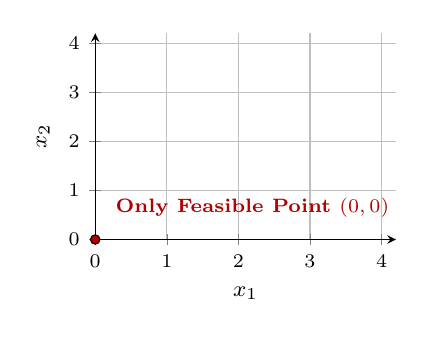
\begin{tikzpicture}
                \begin{axis}[
                    width=5.4cm,
                    height=4.2cm,
                    axis lines=left,
                    xmin=0, xmax=4.2,
                    ymin=0, ymax=4.2,
                    xlabel={$x_1$},
                    ylabel={$x_2$},
                    xtick={0,1,2,3,4},
                    ytick={0,1,2,3,4},
                    tick label style={font=\scriptsize},
                    label style={font=\footnotesize},
                    grid=major,
                    clip=false
                ]
                    \addplot[integer point] coordinates {(0,0)};
                    \node[anchor=south west, font=\scriptsize, red!70!black] at (axis cs:0.15,0.25) {\textbf{Only Feasible Point $(0,0)$}};
                \end{axis}
            \end{tikzpicture}
        \end{column}
    \end{columns}
\end{frame}

% ----------------------------------------------------------------------
% SLIDE 7: MILP Case 2: y = 1
% ----------------------------------------------------------------------
\begin{frame}{Step 4: Solving the MILP -- Case 2}{Case 2: Facility Activated ($y=1$)}
    \footnotesize
    If the company \textbf{pays} the fixed cost ($y=1$), we use the LP optimal found in Step 1.

    \begin{columns}[T]
        \begin{column}{0.50\textwidth}
            \begin{itemize}
                \item \textbf{Fixed Cost Constraint becomes:}
                \[ x_1 + x_2 - 10(1) \le 0 \quad \implies \quad x_1 + x_2 \le 10 \]
                \item This is identical to $C_1$, so the feasible region remains the original shaded polygon.
                \item The optimal production mix is the LP solution:
                \[ \mathbf{x_1^* = 6, \quad x_2^* = 4} \]
                \item \textbf{Total Net Profit ($Z$):}
                \[ Z = 5(6) + 3(4) - 10(1) = 42 - 10 = \mathbf{\$32} \]
            \end{itemize}
        \end{column}
        \begin{column}{0.47\textwidth}
            \centering
            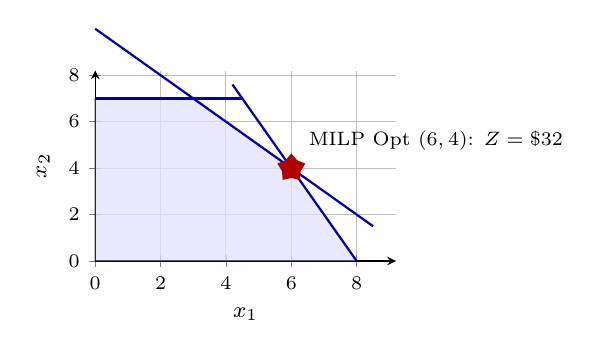
\begin{tikzpicture}
                \begin{axis}[
                    width=5.4cm,
                    height=4.0cm,
                    axis lines=left,
                    xmin=0, xmax=9.2, ymin=0, ymax=8.2,
                    xlabel={$x_1$}, ylabel={$x_2$},
                    xtick={0, 2, 4, 6, 8}, ytick={0, 2, 4, 6, 8},
                    tick label style={font=\scriptsize},
                    label style={font=\footnotesize},
                    grid=major, clip=false
                ]
                \addplot[feasible area] coordinates {(0, 0) (8, 0) (6, 4) (3, 7) (0, 7)} \closedcycle;

                \addplot[constraint line, domain=0:8.5] {10 - x};
                \addplot[constraint line, domain=4.2:8] {16 - 2*x};
                \draw[constraint line] (axis cs:0, 7) -- (axis cs:4.5, 7);

                \coordinate (MILP_Opt) at (axis cs:6, 4);
                \node[milp optimal, label={[font=\scriptsize, anchor=south west]above right:\alert{MILP Opt $(6, 4)$}: $Z=\$32$}] at (MILP_Opt) {};
                \end{axis}
            \end{tikzpicture}
        \end{column}
    \end{columns}
\end{frame}

% ----------------------------------------------------------------------
% SLIDE 8: Conclusion and Optimal Solution
% ----------------------------------------------------------------------
\begin{frame}{Conclusion: The Optimal MILP Solution}{Comparing the Binary Choices}
    \begin{columns}[T]
        \begin{column}{0.50\textwidth}
            \footnotesize
            \begin{itemize}
                \item \textbf{Case 1 (No Capacity):} $y=0 \implies Z = \mathbf{\$0}$
                \item \textbf{Case 2 (Capacity Activated):} $y=1 \implies Z = \mathbf{\$32}$
            \end{itemize}

            \begin{alertblock}{Optimal Decision}
                The optimal profit is $\mathbf{Z^* = \$32}$, achieved in Case 2.
            \end{alertblock}
            \begin{block}{Optimal MILP Solution}
                \begin{itemize}
                    \item $\mathbf{y^* = 1}$ (Activate facility)
                    \item $\mathbf{x_1^* = 6}$ units, $\mathbf{x_2^* = 4}$ units
                \end{itemize}
                The fixed cost (\$10) is outweighed by the gross profit (\$42).
            \end{block}
        \end{column}
        \begin{column}{0.47\textwidth}
            \centering
            \footnotesize \textbf{Visualization of the Two Candidate Optima}\\[2pt]
            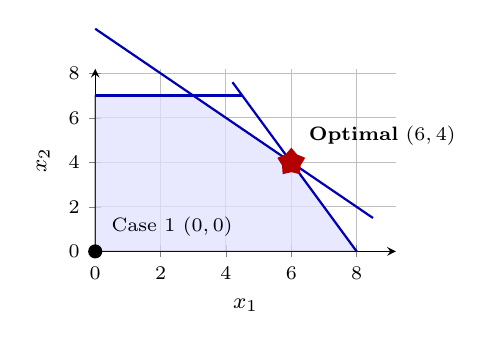
\begin{tikzpicture}
                \begin{axis}[
                    width=5.4cm,
                    height=3.9cm,
                    axis lines=left,
                    xmin=0, xmax=9.2, ymin=0, ymax=8.2,
                    xlabel={$x_1$}, ylabel={$x_2$},
                    xtick={0, 2, 4, 6, 8}, ytick={0, 2, 4, 6, 8},
                    tick label style={font=\scriptsize},
                    label style={font=\footnotesize},
                    grid=major, clip=false
                ]
                \addplot[feasible area] coordinates {(0, 0) (8, 0) (6, 4) (3, 7) (0, 7)} \closedcycle;

                \addplot[constraint line, domain=0:8.5] {10 - x};
                \addplot[constraint line, domain=4.2:8] {16 - 2*x};
                \draw[constraint line] (axis cs:0, 7) -- (axis cs:4.5, 7);

                \coordinate (MILP_Opt) at (axis cs:6, 4);
                \node[milp optimal, label={[font=\scriptsize, anchor=south west]above right:\textbf{Optimal} $(6, 4)$}] at (MILP_Opt) {};
                \node[fixed cost point] at (axis cs:0, 0) {};
                \node[font=\scriptsize, anchor=south west] at (axis cs:0.2, 0.25) {Case 1 $(0,0)$};
                \end{axis}
            \end{tikzpicture}
        \end{column}
    \end{columns}
\end{frame}

% ----------------------------------------------------------------------
% SLIDE: PuLP 4.0 Code for Fixed Setup Cost MILP
% ----------------------------------------------------------------------
\begin{frame}[fragile]{Fixed Setup Cost MILP in Python (PuLP 4.0)}{Example 4: Modeling Big-$M$ Linking Constraints}
\begin{columns}[T]
\begin{column}{0.58\textwidth}
\begin{lstlisting}
import pulp

prob = pulp.LpProblem("Fixed_Setup_Cost_MILP", pulp.LpMaximize)

# Continuous production variables and binary setup variable
x1 = prob.add_variable("x1", lowBound=0, cat=pulp.LpContinuous)
x2 = prob.add_variable("x2", lowBound=0, cat=pulp.LpContinuous)
y  = prob.add_variable("y", cat=pulp.LpBinary)

# Objective: Gross Profit - Fixed Setup Cost
prob += 5 * x1 + 3 * x2 - 10 * y, "Net_Profit"

# Resource constraints + Big-M linking constraint (M = 10)
prob += x1 + x2 <= 10, "Resource_A"
prob += 2 * x1 + x2 <= 16, "Resource_B"
prob += x2 <= 7, "Resource_C"
prob += x1 + x2 - 10 * y <= 0, "Big_M_Link"

res = prob.solve()
z_opt = pulp.value(prob.objective)
print(f"Status: {res.status.name}, Net Profit Z* = ${z_opt:.2f}")
print(f"Activate y*={int(y.varValue)}, x1*={x1.varValue}, x2*={x2.varValue}")
\end{lstlisting}
\end{column}
\begin{column}{0.39\textwidth}
\begin{block}{Console Output}
\footnotesize
\texttt{Status: Optimal}\\
\texttt{Net Profit Z* = \$32.00}\\
\texttt{Activate Facility y* = 1}\\
\texttt{x1* = 6.0, x2* = 4.0}
\end{block}
\begin{alertblock}{Why Big-$M$ Matters}
\scriptsize
Without \texttt{x1 + x2 - 10 * y <= 0}, the solver would set \texttt{y = 0} to avoid the \$10 fee while still producing \texttt{x1 = 6, x2 = 4}!
\end{alertblock}
\end{column}
\end{columns}
\end{frame}


\section{Modeling a Min Purchase Quantity}
\begin{frame}\sectionpage\end{frame}

\begin{frame}{Problem Description: Minimum Purchase Quantity}
\textbf{Context:}
\begin{itemize}
  \item A company can order two products --- A and B --- from a single supplier.
  \item Ordering from the supplier incurs a fixed setup (shipping) cost of \$12.
  \item If an order is placed, the supplier requires a \textbf{minimum purchase quantity (MOQ)} of 6 total units.
  \item Each product consumes limited assembly hours (16 hours available).
  \item The firm must decide whether to place an order at all, and how many units of each product to order.
\end{itemize}

\textbf{Goal:}
\begin{itemize}
  \item Maximize total net profit = profit from A and B $-$ fixed ordering cost.
\end{itemize}
\end{frame}

\begin{frame}{Decision Variables and Parameters}
\textbf{Decision Variables:}
\begin{itemize}
  \item $x_1$ = quantity of Product A to order (units)
  \item $x_2$ = quantity of Product B to order (units)
  \item $y =
  \begin{cases}
  1 & \text{if an order is placed},\\
  0 & \text{otherwise}.
  \end{cases}$
\end{itemize}

\textbf{Parameters:}
\begin{itemize}
  \item Profit per unit: \$7 for A, \$5 for B
  \item Fixed ordering cost: \$12 (incurred only if $y=1$)
  \item Assembly time: 2 hours for A, 1 hour for B (max 16 hours)
  \item Minimum purchase quantity (MOQ): at least 6 total units if an order is placed ($y=1$)
\end{itemize}
\end{frame}

\begin{frame}{MILP with Minimum Purchase Quantity (MOQ)}
\textbf{Focusing on the Switching Constraints:}
\begin{itemize}
  \item Apart from the single resource limit ($2x_1 + x_2 \le 16$), the core integer programming innovation is the pair of \textbf{switching constraints} controlled by $y \in \{0,1\}$:
\end{itemize}

\[
\max \; Z \;=\; 7x_1 + 5x_2 \;-\; 12y
\]
\[
\text{s.t. }\begin{cases}
\text{Assembly hours:} & 2x_1 + x_2 \le 16 \\[4pt]
\textbf{MOQ switch (lower bound):} & \mathbf{x_1 + x_2 \;\ge\; 6\,y} \\[2pt]
\textbf{Big-$M$ switch (upper bound):} & \mathbf{x_1 + x_2 \;\le\; 16\,y} \\[4pt]
x_1, x_2 \in \mathbb{Z}_{\ge 0},\quad \mathbf{y \in \{0,1\}}
\end{cases}
\]

\centering
\alert{\textbf{Two-Sided Switching Rule:}\quad $\mathbf{6y \;\le\; x_1 + x_2 \;\le\; 16y}$}
\begin{itemize}
  \footnotesize
  \item If $y=0$: $0 \le x_1 + x_2 \le 0 \implies x_1 = x_2 = 0$ (no purchase allowed).
  \item If $y=1$: $6 \le x_1 + x_2 \le 16$ (MOQ enforced; $M=16$ is the natural max from $2x_1 + x_2 \le 16$).
\end{itemize}
\end{frame}

% ----------------------------------------------------------------------
% NEW SLIDE: Solving the MOQ Model
% ----------------------------------------------------------------------
\begin{frame}{Solving the MOQ Model: Optimal Solution \& Analysis}{Comparing No-Order ($y=0$) vs. Active Order ($y=1$)}
\begin{columns}[T]
\begin{column}{0.50\textwidth}
  \footnotesize
  \begin{block}{Case 1: Do Not Order ($y=0$)}
    \begin{itemize}
      \item Switching rule $0 \le x_1 + x_2 \le 0$ forces $x_1 = 0, \; x_2 = 0 \implies Z = \mathbf{\$0}$.
    \end{itemize}
  \end{block}
  \begin{block}{Case 2: Place Order ($y=1$)}
    \begin{itemize}
      \item Switching rule becomes $6 \le x_1 + x_2 \le 16$ alongside $2x_1 + x_2 \le 16$.
      \item Profit per assembly hour: Product B earns $\$5/\text{hr}$ vs.\ Product A at $\$7/2 = \$3.50/\text{hr}$.
      \item \textbf{Optimal Solution:} $x_1^* = 0, \; x_2^* = 16, \; y^* = 1$
      \[
        Z^* = 7(0) + 5(16) - 12(1) = \mathbf{\$68.00}.
      \]
    \end{itemize}
  \end{block}
\end{column}
\begin{column}{0.47\textwidth}
  \centering
  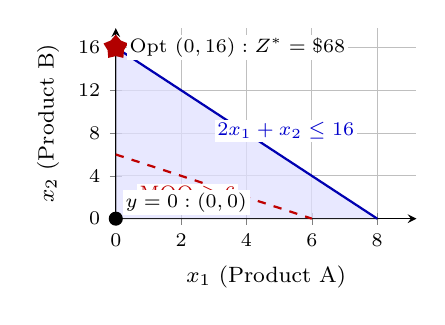
\begin{tikzpicture}
    \begin{axis}[
      width=5.4cm,
      height=4.0cm,
      axis lines=left,
      xmin=0, xmax=9.2, ymin=0, ymax=17.8,
      xlabel={$x_1$ (Product A)}, ylabel={$x_2$ (Product B)},
      xtick={0,2,4,6,8}, ytick={0,4,8,12,16},
      tick label style={font=\scriptsize},
      label style={font=\footnotesize},
      grid=major, clip=false
    ]
      % Feasible region for y=1:
      % x1 + x2 >= 6, 2x1 + x2 <= 16
      % Vertices: (6,0), (8,0), (0,16), (0,6)
      \addplot[feasible area] coordinates {(6,0) (8,0) (0,16) (0,6)} \closedcycle;

      \addplot[constraint line, domain=0:8] {16 - 2*x};
      \node[font=\scriptsize, blue!80!black, fill=white, inner sep=1pt] at (axis cs:5.2, 8.2) {$2x_1 + x_2 \le 16$};

      \addplot[thick, red!75!black, dashed, domain=0:6] {6 - x};
      \node[font=\scriptsize, red!75!black, fill=white, inner sep=1pt] at (axis cs:2.2, 2.2) {MOQ $\ge 6$};

      % Origin (y=0)
      \node[fixed cost point] at (axis cs:0,0) {};
      \node[font=\scriptsize, fill=white, inner sep=1pt, anchor=south west] at (axis cs:0.2,0.3) {$y=0:(0,0)$};

      % Optimal Solution (0, 16)
      \node[ilp optimal, label={[font=\scriptsize, fill=white, inner sep=1pt, anchor=west]right=3pt:Opt $(0, 16): Z^*=\$68$}] at (axis cs:0,16) {};
    \end{axis}
  \end{tikzpicture}
\end{column}
\end{columns}
\end{frame}

% ----------------------------------------------------------------------
% NEW SLIDE: PuLP 4.0 Code for MOQ Model
% ----------------------------------------------------------------------
\begin{frame}[fragile]{Solving the MOQ Model in Python (PuLP 4.0)}{Example 5: Disjunctive Feasible Region with Switching Constraints}
\begin{columns}[T]
\begin{column}{0.58\textwidth}
\begin{lstlisting}
import pulp

prob = pulp.LpProblem("Supplier_Order_MOQ", pulp.LpMaximize)

# Integer order quantities x1, x2 and binary order indicator y
x1 = prob.add_variable("x1", lowBound=0, cat=pulp.LpInteger)
x2 = prob.add_variable("x2", lowBound=0, cat=pulp.LpInteger)
y  = prob.add_variable("y", cat=pulp.LpBinary)

prob += 7 * x1 + 5 * x2 - 12 * y, "Net_Profit"

# Single resource constraint
prob += 2 * x1 + x2 <= 16, "Assembly_Hours"

# Two-sided switching constraints: 6*y <= x1 + x2 <= 16*y
prob += x1 + x2 - 6 * y >= 0, "MOQ_Lower_Switch"
prob += x1 + x2 - 16 * y <= 0, "Big_M_Upper_Switch"

res = prob.solve()
z_opt = pulp.value(prob.objective)
print(f"Status: {res.status.name}, Profit Z* = ${z_opt:.2f}")
print(f"y*={y.varValue:.0f}, x1*={x1.varValue:.0f}, x2*={x2.varValue:.0f}")
\end{lstlisting}
\end{column}
\begin{column}{0.39\textwidth}
\begin{block}{Console Output}
\footnotesize
\texttt{Status: Optimal}\\
\texttt{Profit Z* = \$68.00}\\
\texttt{Order y* = 1}\\
\texttt{x1* = 0, x2* = 16}
\end{block}
\begin{alertblock}{Modeling Insight}
\scriptsize
Combining $\mathbf{x_1 + x_2 \ge 6y}$ with $\mathbf{x_1 + x_2 \le 16y}$ creates a \textit{semi-continuous} switch: total quantity is either \textbf{0} ($y=0$) or \textbf{between 6 and 16} ($y=1$).
\end{alertblock}
\end{column}
\end{columns}
\end{frame}


% ======================================================================
% SECTION: Fixed-Charge Transshipment Problem
% ======================================================================
\section{Fixed-Charge Transshipment Problem}
\begin{frame}\sectionpage\end{frame}

% ----------------------------------------------------------------------
% SLIDE 42: Problem Setup & Network Diagram
% ----------------------------------------------------------------------
\begin{frame}{Fixed-Charge Transshipment Problem}{Warehouse Selection and Network Flow}
\begin{columns}[T,onlytextwidth]
\begin{column}{0.51\textwidth}
  \footnotesize
  \textbf{Logistics Network Setup:}
  \begin{itemize}\setlength{\itemsep}{2pt}
    \item \textbf{3 Candidate Warehouses ($W_1, W_2, W_3$):} Each holds $S_i = 50$ units. Shipping any positive volume from $W_i$ incurs a \textbf{fixed setup/dispatch fee $F_i$}.
    \item \textbf{Central Transshipment Hub ($T$):} Consolidates all inbound shipments ($\text{Flow In} = \text{Flow Out}$) and forwards them to Customer $D$ at $\$3/\text{unit}$.
    \item \textbf{Customer Sink ($D$):} Requires exactly $80$ units.
  \end{itemize}
  \vspace{2pt}
  \centering
  {\scriptsize\setlength{\tabcolsep}{3.5pt}
  \begin{tabular}{@{}lccc@{}}
    \toprule
    \textbf{Warehouse} & \textbf{Supply ($S_i$)} & \textbf{Fixed Fee ($F_i$)} & \textbf{Cost ($c_{iT}$)} \\
    \midrule
    $W_1$ (North)   & $50$ units & $\$120$ & $\$2/\text{unit}$ \\
    $W_2$ (Central) & $50$ units & $\$70$  & $\$4/\text{unit}$ \\
    $W_3$ (South)   & $50$ units & $\$50$  & $\$5/\text{unit}$ \\
    \bottomrule
  \end{tabular}}
\end{column}
\begin{column}{0.46\textwidth}
  \centering
  \vspace{4pt}
  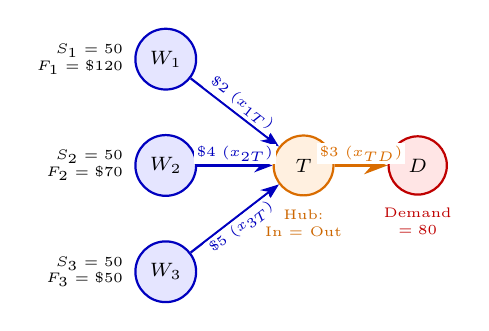
\begin{tikzpicture}[>=Stealth, every node/.style={font=\scriptsize}]
    % Warehouse nodes
    \node[circle, draw=blue!75!black, thick, fill=blue!10, minimum size=0.72cm] (W1) at (0, 1.35) {\textbf{$W_1$}};
    \node[circle, draw=blue!75!black, thick, fill=blue!10, minimum size=0.72cm] (W2) at (0, 0)    {\textbf{$W_2$}};
    \node[circle, draw=blue!75!black, thick, fill=blue!10, minimum size=0.72cm] (W3) at (0,-1.35) {\textbf{$W_3$}};

    % Supply & Fixed cost labels on left
    \node[anchor=east, align=right, font=\tiny] at (-0.42, 1.35) {$S_1=50$\\$F_1=\$120$};
    \node[anchor=east, align=right, font=\tiny] at (-0.42, 0)    {$S_2=50$\\$F_2=\$70$};
    \node[anchor=east, align=right, font=\tiny] at (-0.42,-1.35) {$S_3=50$\\$F_3=\$50$};

    % Transshipment Hub
    \node[circle, draw=orange!85!black, thick, fill=orange!12, minimum size=0.76cm] (T) at (1.75, 0) {\textbf{$T$}};
    \node[anchor=north, align=center, font=\tiny, orange!80!black] at (1.75, -0.44) {Hub:\\In $=$ Out};

    % Sink Node
    \node[circle, draw=red!75!black, thick, fill=red!10, minimum size=0.74cm] (D) at (3.20, 0) {\textbf{$D$}};
    \node[anchor=north, align=center, font=\tiny, red!75!black] at (3.20, -0.42) {Demand\\$= 80$};

    % Directed Arcs
    \draw[->, thick, blue!75!black] (W1) -- (T) node[midway, above, sloped, font=\tiny, fill=white, inner sep=1pt] {$\$2$ ($x_{1T}$)};
    \draw[->, thick, blue!75!black] (W2) -- (T) node[midway, above, font=\tiny, fill=white, inner sep=1pt] {$\$4$ ($x_{2T}$)};
    \draw[->, thick, blue!75!black] (W3) -- (T) node[midway, below, sloped, font=\tiny, fill=white, inner sep=1pt] {$\$5$ ($x_{3T}$)};
    \draw[->, very thick, orange!85!black] (T) -- (D) node[midway, above, font=\tiny, fill=white, inner sep=1pt] {$\$3$ ($x_{TD}$)};
  \end{tikzpicture}
\end{column}
\end{columns}
\end{frame}

% ----------------------------------------------------------------------
% SLIDE 43: Decision Variables and Warehouse Activation
% ----------------------------------------------------------------------
\begin{frame}{Decision Variables and Warehouse Activation}{Linking Continuous Network Flows to Binary Setup Choices}
\begin{columns}[T,onlytextwidth]
\begin{column}{0.48\textwidth}
  \begin{block}{1. Continuous Flow Variables ($x_{ij} \ge 0$)}
    \scriptsize
    \begin{itemize}\setlength{\itemsep}{2pt}
      \item $x_{1T}, x_{2T}, x_{3T} \ge 0$: Units shipped from Warehouse $W_1, W_2, W_3$ to Hub $T$.
      \item $x_{TD} \ge 0$: Consolidated units shipped from Hub $T$ to Customer $D$.
    \end{itemize}
  \end{block}
  \begin{block}{2. Binary Activation Variables ($y_i \in \{0,1\}$)}
    \scriptsize
    \begin{itemize}\setlength{\itemsep}{2pt}
      \item $y_i = 1$ if Warehouse $W_i$ is opened/used ($i=1,2,3$), and $y_i = 0$ otherwise.
    \end{itemize}
  \end{block}
\end{column}
\begin{column}{0.48\textwidth}
  \begin{alertblock}{Big-$M$ Capacity \& Activation Rule}
    \scriptsize
    Each warehouse's inventory ($S_i = 50$) serves as the exact Big-$M$ upper bound:
    \[
      \mathbf{x_{iT} \le 50 y_i \iff x_{iT} - 50 y_i \le 0} \quad (i=1,2,3)
    \]
    \begin{itemize}\setlength{\itemsep}{1pt}
      \item $y_i = 0 \implies x_{iT} = 0$ (no flow without paying $F_i$).
      \item $y_i = 1 \implies x_{iT} \le 50$ (full capacity unlocked).
    \end{itemize}
  \end{alertblock}
  \begin{exampleblock}{Transshipment Hub Conservation ($T$)}
    \scriptsize
    Hub $T$ holds no inventory ($\text{Flow In} = \text{Flow Out}$):
    \[
      \mathbf{x_{1T} + x_{2T} + x_{3T} - x_{TD} = 0}
    \]
  \end{exampleblock}
\end{column}
\end{columns}
\end{frame}

% ----------------------------------------------------------------------
% SLIDE 44: Complete MILP Formulation
% ----------------------------------------------------------------------
\begin{frame}{MILP Formulation: Fixed-Charge Transshipment}{Combining Fixed Setup Fees, Big-$M$ Capacities, and Flow Balance}
  \footnotesize
  \[
    \min \quad Z = \underbrace{120y_1 + 70y_2 + 50y_3}_{\text{Fixed Warehouse Setup Fees}} + \underbrace{2x_{1T} + 4x_{2T} + 5x_{3T} + 3x_{TD}}_{\text{Variable Transshipment Costs}}
  \]
  \textbf{Subject to:}
  \begin{align*}
    x_{1T} - 50y_1 &\le 0 && \text{(Warehouse 1 Capacity \& Activation)} \\
    x_{2T} - 50y_2 &\le 0 && \text{(Warehouse 2 Capacity \& Activation)} \\
    x_{3T} - 50y_3 &\le 0 && \text{(Warehouse 3 Capacity \& Activation)} \\[3pt]
    x_{1T} + x_{2T} + x_{3T} - x_{TD} &= 0 && \text{(Flow Conservation at Hub } T\text{)} \\
    x_{TD} &= 80 && \text{(Demand Requirement at Sink } D\text{)} \\[3pt]
    x_{1T}, x_{2T}, x_{3T}, x_{TD} &\ge 0, \quad y_1, y_2, y_3 \in \{0, 1\}
  \end{align*}
\end{frame}

% ----------------------------------------------------------------------
% SLIDE 45: Optimal Solution & Cost Trade-Off
% ----------------------------------------------------------------------
\begin{frame}{Optimal Solution: Fixed vs.\ Variable Cost Trade-Off}{Why the Cheapest Setup Fee Does Not Win}
\vspace{-0.3em}
\begin{columns}[T,onlytextwidth]
\begin{column}{0.51\textwidth}
  \scriptsize
  Since each warehouse holds $50$ units and demand is $80$ units, \textbf{at least two warehouses} must open:
  \begin{block}{1. Cheapest Setup Pair $\{W_2, W_3\}$ ($y_2=1, y_3=1$)}
    $x_{2T}=50, \; x_{3T}=30, \; x_{TD}=80$\\
    Fixed $\$120 + \text{Var } \$590 \implies \text{Total Cost} = \mathbf{\$710}$.
  \end{block}
  \vspace{-0.3em}
  \begin{block}{2. Mixed Pair $\{W_1, W_3\}$ ($y_1=1, y_3=1$)}
    $x_{1T}=50, \; x_{3T}=30, \; x_{TD}=80$\\
    Fixed $\$170 + \text{Var } \$490 \implies \text{Total Cost} = \mathbf{\$660}$.
  \end{block}
  \vspace{-0.3em}
  \begin{exampleblock}{3. Optimal MILP Pair $\{W_1, W_2\}$ ($y_1^*=1, y_2^*=1, y_3^*=0$)}
    $x_{1T}^*=50, \; x_{2T}^*=30, \; x_{3T}^*=0, \; x_{TD}^*=80$\\
    Fixed $\$190 + \text{Var } \$460 \implies \text{Optimal } \mathbf{Z^* = \$650}$.
  \end{exampleblock}
\end{column}
\begin{column}{0.46\textwidth}
  \centering
  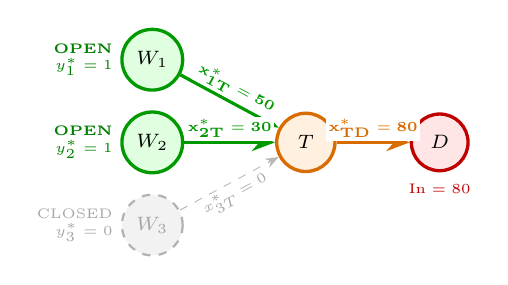
\begin{tikzpicture}[>=Stealth, every node/.style={font=\scriptsize}]
    % Active W1 & W2, Inactive W3
    \node[circle, draw=green!60!black, very thick, fill=green!12, minimum size=0.68cm] (W1) at (0, 1.05) {\textbf{$W_1$}};
    \node[circle, draw=green!60!black, very thick, fill=green!12, minimum size=0.68cm] (W2) at (0, 0)    {\textbf{$W_2$}};
    \node[circle, draw=gray!60, dashed, thick, fill=gray!10, text=gray!70, minimum size=0.68cm] (W3) at (0,-1.05) {\textbf{$W_3$}};

    \node[anchor=east, align=right, font=\tiny, green!50!black] at (-0.38, 1.05) {\textbf{OPEN}\\$y_1^*=1$};
    \node[anchor=east, align=right, font=\tiny, green!50!black] at (-0.38, 0)    {\textbf{OPEN}\\$y_2^*=1$};
    \node[anchor=east, align=right, font=\tiny, gray!70]        at (-0.38,-1.05) {CLOSED\\$y_3^*=0$};

    \node[circle, draw=orange!85!black, very thick, fill=orange!12, minimum size=0.74cm] (T) at (1.95, 0) {\textbf{$T$}};
    \node[circle, draw=red!75!black, very thick, fill=red!10, minimum size=0.72cm] (D) at (3.65, 0) {\textbf{$D$}};
    \node[anchor=north, font=\tiny, red!75!black] at (3.65, -0.40) {$\text{In} = 80$};

    % Active & Inactive Arcs
    \draw[->, very thick, green!60!black] (W1) -- (T) node[midway, above, sloped, font=\tiny, fill=white, inner sep=1pt] {$\mathbf{x_{1T}^*=50}$};
    \draw[->, very thick, green!60!black] (W2) -- (T) node[midway, above, font=\tiny, fill=white, inner sep=1pt] {$\mathbf{x_{2T}^*=30}$};
    \draw[->, dashed, gray!55]            (W3) -- (T) node[midway, below, sloped, font=\tiny, text=gray!70, fill=white, inner sep=1pt] {$x_{3T}^*=0$};
    \draw[->, very thick, orange!85!black] (T) -- (D) node[midway, above, font=\tiny, fill=white, inner sep=1pt] {$\mathbf{x_{TD}^*=80}$};
  \end{tikzpicture}
  \vspace{-0.2em}
  \begin{alertblock}{Economic Intuition}
    \scriptsize
    Opening $W_1$ costs $\$70$ more in fixed fees than $W_3$, but saves $(\$5-\$2)\times 50 = \mathbf{\$150}$ in shipping—netting $\mathbf{\$60}$ over $\{W_2, W_3\}$!
  \end{alertblock}
\end{column}
\end{columns}
\end{frame}

% ----------------------------------------------------------------------
% SLIDE 46: PuLP 4.0 Implementation
% ----------------------------------------------------------------------
\begin{frame}[fragile]{Fixed-Charge Transshipment in Python (PuLP 4.0)}{Example 6: Network Flow Conservation with Binary Setup Variables}
\begin{columns}[T]
\begin{column}{0.58\textwidth}
\begin{lstlisting}
import pulp

prob = pulp.LpProblem("Fixed_Charge_Transshipment", pulp.LpMinimize)
x1T = prob.add_variable("x1T", lowBound=0, cat=pulp.LpContinuous)
x2T = prob.add_variable("x2T", lowBound=0, cat=pulp.LpContinuous)
x3T = prob.add_variable("x3T", lowBound=0, cat=pulp.LpContinuous)
xTD = prob.add_variable("xTD", lowBound=0, cat=pulp.LpContinuous)
y1  = prob.add_variable("y1", cat=pulp.LpBinary)
y2  = prob.add_variable("y2", cat=pulp.LpBinary)
y3  = prob.add_variable("y3", cat=pulp.LpBinary)

prob += 120*y1 + 70*y2 + 50*y3 + 2*x1T + 4*x2T + 5*x3T + 3*xTD
prob += x1T - 50 * y1 <= 0, "Cap_W1"
prob += x2T - 50 * y2 <= 0, "Cap_W2"
prob += x3T - 50 * y3 <= 0, "Cap_W3"
prob += x1T + x2T + x3T - xTD == 0, "Hub_T_Balance"
prob += xTD == 80, "Sink_D_Demand"

res = prob.solve()
print(f"Status: {res.status.name}, Cost Z* = ${pulp.value(prob.objective):.2f}")
print(f"Open: y1={y1.varValue:.0f}, y2={y2.varValue:.0f}, y3={y3.varValue:.0f}")
print(f"Flow: x1T={x1T.varValue:.0f}, x2T={x2T.varValue:.0f}, xTD={xTD.varValue:.0f}")
\end{lstlisting}
\end{column}
\begin{column}{0.39\textwidth}
\begin{block}{Console Output}
\footnotesize
\texttt{Status: Optimal}\\
\texttt{Cost Z* = \$650.00}\\
\texttt{Open: y1=1, y2=1, y3=0}\\
\texttt{Flow: x1T=50, x2T=30, xTD=80}
\end{block}
\begin{alertblock}{LP Relaxation Trap}
\scriptsize
If $y_i$ were relaxed to continuous $0 \le y_i \le 1$, the solver would set $y_2 = 30/50 = 0.6$ to pay only $60\%$ of $W_2$'s fixed fee ($Z_{\text{LP}} = \$622.00$). Enforcing \texttt{LpBinary} ensures full setup fees are paid!
\end{alertblock}
\end{column}
\end{columns}
\end{frame}


% ======================================================================
% SECTION: Store Location Problem (Set Covering)
% ======================================================================
\section{Store Location Problem (Set Covering)}
\begin{frame}\sectionpage\end{frame}

% ----------------------------------------------------------------------
% SLIDE 48: Problem Setup & City Grid Diagram
% ----------------------------------------------------------------------
\begin{frame}{Store Location on a City Grid}{The Set Covering Problem}
\begin{columns}[T,onlytextwidth]
\begin{column}{0.51\textwidth}
  \scriptsize
  \textbf{Retail Network Coverage Problem:}
  \begin{itemize}\setlength{\itemsep}{1.5pt}
    \item A retail chain is entering a city divided into a \textbf{$2 \times 3$ grid of 6 sectors} ($1, \dots, 6$).
    \item Opening a store in Sector $j$ serves customers in \textbf{Sector $j$ itself} plus all \textbf{orthogonally adjacent sectors} (sharing a horizontal or vertical border; diagonals do not count).
    \item \textbf{Goal:} Open the \textbf{minimum number of stores} so every sector is covered by \emph{at least one} store.
  \end{itemize}
  \vspace{2pt}
  \centering
  {\scriptsize\setlength{\tabcolsep}{4pt}
  \begin{tabular}{@{}cl@{}}
    \toprule
    \textbf{Sector $i$} & \textbf{Adjacent Neighborhood $N(i)$ (Can Cover $i$)} \\
    \midrule
    Sector 1 & $\{1, 2, 4\}$ \\
    Sector 2 & $\{1, 2, 3, 5\}$ \\
    Sector 3 & $\{2, 3, 6\}$ \\
    Sector 4 & $\{1, 4, 5\}$ \\
    Sector 5 & $\{2, 4, 5, 6\}$ \\
    Sector 6 & $\{3, 5, 6\}$ \\
    \bottomrule
  \end{tabular}}
\end{column}
\begin{column}{0.46\textwidth}
  \centering
  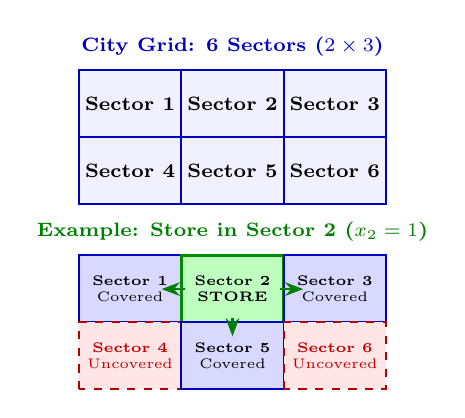
\begin{tikzpicture}[every node/.style={font=\scriptsize}]
    % Top Grid: City Map
    \node[font=\scriptsize\bfseries, blue!75!black] at (1.95, 2.05) {City Grid: 6 Sectors ($2 \times 3$)};
    \foreach \col/\sec in {0/1, 1/2, 2/3} {
      \draw[thick, draw=blue!75!black, fill=blue!6] (\col*1.3, 0.9) rectangle ++(1.3, 0.85)
        node[pos=0.5, align=center] {\textbf{Sector \sec}};
    }
    \foreach \col/\sec in {0/4, 1/5, 2/6} {
      \draw[thick, draw=blue!75!black, fill=blue!6] (\col*1.3, 0.05) rectangle ++(1.3, 0.85)
        node[pos=0.5, align=center] {\textbf{Sector \sec}};
    }

    % Bottom Grid: Example Coverage from Sector 2
    \begin{scope}[yshift=-2.35cm]
      \node[font=\scriptsize\bfseries, green!50!black] at (1.95, 2.05) {Example: Store in Sector 2 ($x_2 = 1$)};
      % Sector 1 (covered)
      \draw[thick, draw=blue!75!black, fill=blue!15] (0, 0.9) rectangle ++(1.3, 0.85)
        node[pos=0.5, align=center, font=\tiny] {\textbf{Sector 1}\\Covered};
      % Sector 2 (store)
      \draw[very thick, draw=green!55!black, fill=green!25] (1.3, 0.9) rectangle ++(1.3, 0.85)
        node[pos=0.5, align=center, font=\tiny] {\textbf{Sector 2}\\\textbf{STORE}};
      % Sector 3 (covered)
      \draw[thick, draw=blue!75!black, fill=blue!15] (2.6, 0.9) rectangle ++(1.3, 0.85)
        node[pos=0.5, align=center, font=\tiny] {\textbf{Sector 3}\\Covered};
      % Sector 4 (uncovered)
      \draw[thick, dashed, draw=red!70!black, fill=red!10] (0, 0.05) rectangle ++(1.3, 0.85)
        node[pos=0.5, align=center, font=\tiny, red!75!black] {\textbf{Sector 4}\\Uncovered};
      % Sector 5 (covered)
      \draw[thick, draw=blue!75!black, fill=blue!15] (1.3, 0.05) rectangle ++(1.3, 0.85)
        node[pos=0.5, align=center, font=\tiny] {\textbf{Sector 5}\\Covered};
      % Sector 6 (uncovered)
      \draw[thick, dashed, draw=red!70!black, fill=red!10] (2.6, 0.05) rectangle ++(1.3, 0.85)
        node[pos=0.5, align=center, font=\tiny, red!75!black] {\textbf{Sector 6}\\Uncovered};

      % Coverage arrows from Sector 2
      \draw[-Stealth, thick, green!50!black] (1.35, 1.32) -- (1.05, 1.32);
      \draw[-Stealth, thick, green!50!black] (2.55, 1.32) -- (2.85, 1.32);
      \draw[-Stealth, thick, green!50!black] (1.95, 0.95) -- (1.95, 0.72);
    \end{scope}
  \end{tikzpicture}
\end{column}
\end{columns}
\end{frame}

% ----------------------------------------------------------------------
% SLIDE 49: Binary Decision Variables and Coverage Logic
% ----------------------------------------------------------------------
\begin{frame}{Binary Decision Variables and Coverage Logic}{Translating Grid Adjacency into Linear Inequalities}
\begin{columns}[T,onlytextwidth]
\begin{column}{0.48\textwidth}
  \begin{block}{1. Binary Location Variables ($x_j \in \{0,1\}$)}
    \scriptsize
    For each grid sector $j \in \{1, 2, 3, 4, 5, 6\}$:
    \[
      x_j = \begin{cases}
        1 & \text{if a store is opened in Sector } j, \\
        0 & \text{otherwise.}
      \end{cases}
    \]
  \end{block}
  \begin{block}{2. Objective Function}
    \scriptsize
    Minimize the total number of stores opened across the city:
    \[
      \min \quad Z = \sum_{j=1}^6 x_j = x_1 + x_2 + x_3 + x_4 + x_5 + x_6
    \]
  \end{block}
\end{column}
\begin{column}{0.48\textwidth}
  \begin{alertblock}{3. Set Covering Constraint Rule}
    \scriptsize
    Every sector $i \in \{1,\dots,6\}$ must have \textbf{at least one} open store within its neighborhood $N(i)$:
    \[
      \mathbf{\sum_{j \in N(i)} x_j \ge 1 \quad \forall i \in \{1,\dots,6\}}
    \]
  \end{alertblock}
  \begin{exampleblock}{Examples of Sector Coverage Constraints}
    \scriptsize
    \begin{itemize}\setlength{\itemsep}{2pt}
      \item \textbf{Sector 1} ($N(1) = \{1, 2, 4\}$):
        \[
          x_1 + x_2 + x_4 \ge 1
        \]
      \item \textbf{Sector 2} ($N(2) = \{1, 2, 3, 5\}$):
        \[
          x_1 + x_2 + x_3 + x_5 \ge 1
        \]
    \end{itemize}
  \end{exampleblock}
\end{column}
\end{columns}
\end{frame}

% ----------------------------------------------------------------------
% SLIDE 50: Complete 0-1 ILP Formulation
% ----------------------------------------------------------------------
\begin{frame}{Complete 0-1 ILP Formulation: Grid Store Location}{Set Covering Model for All Six Sectors}
  \footnotesize
  \[
    \min \quad Z = x_1 + x_2 + x_3 + x_4 + x_5 + x_6
  \]
  \textbf{Subject to (One Coverage Constraint per Sector):}
  \begin{alignat*}{7}
    x_1 &+ x_2 &      &      &+ x_4 &      &      &\ge 1 &\quad &\text{(Cover Sector 1: } \{1,2,4\}\text{)} \\
    x_1 &+ x_2 &+ x_3 &      &      &+ x_5 &      &\ge 1 &\quad &\text{(Cover Sector 2: } \{1,2,3,5\}\text{)} \\
        &  x_2 &+ x_3 &      &      &      &+ x_6 &\ge 1 &\quad &\text{(Cover Sector 3: } \{2,3,6\}\text{)} \\
    x_1 &      &      &+ x_4 &+ x_5 &      &      &\ge 1 &\quad &\text{(Cover Sector 4: } \{1,4,5\}\text{)} \\
        &  x_2 &      &+ x_4 &+ x_5 &+ x_6 &      &\ge 1 &\quad &\text{(Cover Sector 5: } \{2,4,5,6\}\text{)} \\
        &      &  x_3 &      &      &+ x_5 &+ x_6 &\ge 1 &\quad &\text{(Cover Sector 6: } \{3,5,6\}\text{)}
  \end{alignat*}
  \[
    x_1, x_2, x_3, x_4, x_5, x_6 \in \{0, 1\}
  \]
  \vspace{-0.4em}
  \begin{block}{Why $\ge 1$ Instead of $= 1$?}
    \scriptsize
    Using $\ge 1$ (\emph{Set Covering}) allows overlapping coverage when convenient; forcing $= 1$ (\emph{Exact Set Partitioning}) would forbid a sector from bordering two open stores!
  \end{block}
\end{frame}

% ----------------------------------------------------------------------
% SLIDE 51: Optimal Solution & Visual Coverage Maps
% ----------------------------------------------------------------------
\begin{frame}{Optimal Solution: Covering the Grid with Two Stores}{Analyzing Optimal Store Placements ($Z^* = 2$)}
\begin{columns}[T,onlytextwidth]
\begin{column}{0.51\textwidth}
  \scriptsize
  \vspace{-4pt}
  \begin{alertblock}{Why 1 Store Is Impossible ($Z \ge 2$)}
    Central Sectors $2$ and $5$ cover $|N(i)| = 4$ sectors each. Since $4 < 6$, \textbf{no single store can cover all 6 sectors}.
  \end{alertblock}
  \vspace{-5pt}
  \begin{exampleblock}{Optimal Solution A: Central Spine $\{2, 5\}$}
    \begin{itemize}\setlength{\itemsep}{0pt}
      \item Set $\mathbf{x_2^* = 1, \; x_5^* = 1}$ (all other $x_j^* = 0 \implies \mathbf{Z^* = 2}$).
      \item Store 2 covers $\{1, 2, 3, 5\}$; Store 5 covers $\{2, 4, 5, 6\}$.
      \item Union $= \{1,\dots,6\}$ (Sectors $2$ \& $5$ have \emph{double coverage}).
    \end{itemize}
  \end{exampleblock}
  \vspace{-5pt}
  \begin{block}{Optimal Solution B: Opposite Corners $\{1, 6\}$ or $\{3, 4\}$}
    \begin{itemize}\setlength{\itemsep}{0pt}
      \item Set $\mathbf{x_1^* = 1, \; x_6^* = 1}$ (or $\mathbf{x_3^* = 1, \; x_4^* = 1}$) $\implies \mathbf{Z^* = 2}$.
      \item Store 1 covers $\{1, 2, 4\}$; Store 6 covers $\{3, 5, 6\}$ (zero overlap).
    \end{itemize}
  \end{block}
\end{column}
\begin{column}{0.46\textwidth}
  \centering
  \vspace{-2pt}
  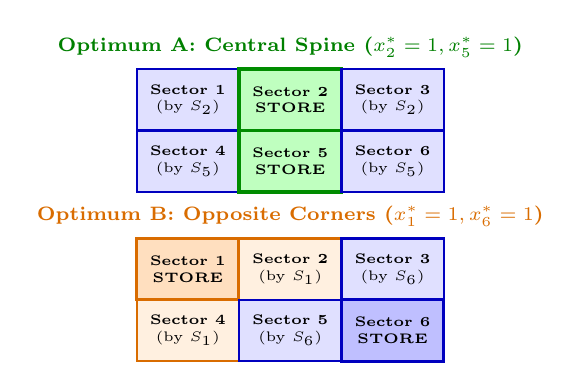
\begin{tikzpicture}[every node/.style={font=\scriptsize}]
    % Top Grid: Central Spine {2, 5}
    \node[font=\scriptsize\bfseries, green!50!black] at (1.95, 1.94) {Optimum A: Central Spine ($x_2^*=1, x_5^*=1$)};
    \draw[thick, draw=blue!75!black, fill=blue!12] (0, 0.88) rectangle ++(1.3, 0.78)
      node[pos=0.5, align=center, font=\tiny] {\textbf{Sector 1}\\(by $S_2$)};
    \draw[very thick, draw=green!55!black, fill=green!25] (1.3, 0.88) rectangle ++(1.3, 0.78)
      node[pos=0.5, align=center, font=\tiny] {\textbf{Sector 2}\\\textbf{STORE}};
    \draw[thick, draw=blue!75!black, fill=blue!12] (2.6, 0.88) rectangle ++(1.3, 0.78)
      node[pos=0.5, align=center, font=\tiny] {\textbf{Sector 3}\\(by $S_2$)};
    \draw[thick, draw=blue!75!black, fill=blue!12] (0, 0.10) rectangle ++(1.3, 0.78)
      node[pos=0.5, align=center, font=\tiny] {\textbf{Sector 4}\\(by $S_5$)};
    \draw[very thick, draw=green!55!black, fill=green!25] (1.3, 0.10) rectangle ++(1.3, 0.78)
      node[pos=0.5, align=center, font=\tiny] {\textbf{Sector 5}\\\textbf{STORE}};
    \draw[thick, draw=blue!75!black, fill=blue!12] (2.6, 0.10) rectangle ++(1.3, 0.78)
      node[pos=0.5, align=center, font=\tiny] {\textbf{Sector 6}\\(by $S_5$)};

    % Bottom Grid: Opposite Corners {1, 6}
    \begin{scope}[yshift=-2.15cm]
      \node[font=\scriptsize\bfseries, orange!85!black] at (1.95, 1.94) {Optimum B: Opposite Corners ($x_1^*=1, x_6^*=1$)};
      \draw[very thick, draw=orange!85!black, fill=orange!25] (0, 0.88) rectangle ++(1.3, 0.78)
        node[pos=0.5, align=center, font=\tiny] {\textbf{Sector 1}\\\textbf{STORE}};
      \draw[thick, draw=orange!85!black, fill=orange!12] (1.3, 0.88) rectangle ++(1.3, 0.78)
        node[pos=0.5, align=center, font=\tiny] {\textbf{Sector 2}\\(by $S_1$)};
      \draw[thick, draw=blue!75!black, fill=blue!12] (2.6, 0.88) rectangle ++(1.3, 0.78)
        node[pos=0.5, align=center, font=\tiny] {\textbf{Sector 3}\\(by $S_6$)};
      \draw[thick, draw=orange!85!black, fill=orange!12] (0, 0.10) rectangle ++(1.3, 0.78)
        node[pos=0.5, align=center, font=\tiny] {\textbf{Sector 4}\\(by $S_1$)};
      \draw[thick, draw=blue!75!black, fill=blue!12] (1.3, 0.10) rectangle ++(1.3, 0.78)
        node[pos=0.5, align=center, font=\tiny] {\textbf{Sector 5}\\(by $S_6$)};
      \draw[very thick, draw=blue!75!black, fill=blue!25] (2.6, 0.10) rectangle ++(1.3, 0.78)
        node[pos=0.5, align=center, font=\tiny] {\textbf{Sector 6}\\\textbf{STORE}};
    \end{scope}
  \end{tikzpicture}
\end{column}
\end{columns}
\end{frame}

% ----------------------------------------------------------------------
% SLIDE 52: PuLP 4.0 Implementation
% ----------------------------------------------------------------------
\begin{frame}[fragile]{Store Location Set Covering in Python (PuLP 4.0)}{Example 7: Dictionary-Driven Neighborhood Coverage Model}
\begin{columns}[T]
\begin{column}{0.58\textwidth}
\begin{lstlisting}
import pulp

prob = pulp.LpProblem("City_Grid_Set_Covering", pulp.LpMinimize)

sectors = [1, 2, 3, 4, 5, 6]
neighbors = {
    1: [1, 2, 4],    2: [1, 2, 3, 5], 3: [2, 3, 6],
    4: [1, 4, 5],    5: [2, 4, 5, 6], 6: [3, 5, 6],
}

# Binary store location variables x[1] .. x[6]
x = {j: prob.add_variable(f"x_{j}", cat=pulp.LpBinary) for j in sectors}

# Objective: Minimize total number of stores opened
prob += sum(x[j] for j in sectors), "Total_Stores"

# Coverage constraint for each sector i
for i in sectors:
    prob += sum(x[j] for j in neighbors[i]) >= 1, f"Cover_Sector_{i}"

res = prob.solve()
chosen = [j for j in sectors if x[j].varValue > 0.5]
print(f"Status: {res.status.name}, Min Stores Z* = {pulp.value(prob.objective):.0f}")
print(f"Open Stores in Sectors: {chosen}")
\end{lstlisting}
\end{column}
\begin{column}{0.39\textwidth}
\begin{block}{Console Output}
\footnotesize
\texttt{Status: Optimal}\\
\texttt{Min Stores Z* = 2}\\
\texttt{Open Stores in Sectors:}\\
\texttt{[3, 4]} \textit{(or \texttt{[2, 5]} / \texttt{[1, 6]})}
\end{block}
\begin{alertblock}{Modeling Scalability}
\scriptsize
By storing adjacency lists in a Python dictionary \texttt{neighbors[i]}, the exact same \texttt{for}-loop scales effortlessly from a 6-sector grid to a 500-zip-code metropolitan network!
\end{alertblock}
\end{column}
\end{columns}
\end{frame}


\begin{frame}{Conclusion}
\begin{itemize}
\item \textbf{Computational Complexity:} ILPs are $\mathcal{NP}$-hard in general; solving an ILP requires solving a sequence of LP relaxations via Branch-and-Bound and Cutting Planes.
\item \textbf{Solver Ecosystem:} Industrial-scale commercial MILP solvers (e.g., Gurobi, CPLEX) are expensive, whereas open-source MILP solvers like \textbf{CBC} (bundled free with Python's \texttt{PuLP}) solve small-to-medium ILPs effectively.
\item \textbf{Duality \& Sensitivity:} Standard LP shadow prices and reduced costs do \textbf{not} directly apply to ILPs because discrete jumps break continuity.
\item \textbf{Core Applications:} 0-1 selection problems (knapsack, assignment, set covering / store location), logical conditions, fixed setup costs, minimum order quantities (MOQ), and fixed-charge transshipment networks.
\end{itemize}
\end{frame}

\end{document}
